
% \documentclass[10pt, pre, twocolumn, showpacs, aps]{revtex4-1}
%\documentclass{iopart}
% \usepackage{amsmath,amssymb}
% \usepackage[dvipdfmx]{graphicx,color}
%\usepackage{graphicx,color}
% \usepackage{ulem}
% \usepackage{pgf,tikz}
% \usepackage{here}
% \usepackage{comment}

% \newcommand{\red}[1]{\textcolor{red}{#1}}
% \newcommand{\blue}[1]{\textcolor{blue}{#1}}
% \newcommand{\magenta}[1]{\textcolor{magenta}{#1}}
% $\newcommand{\remove}[1]{\red{\sout{#1}}}
% \newcommand{\correct}[2]{\red{\sout{#1}}~\red{#2}}


% \begin{document}
\begin{comment}
\title
  {Classification of bifurcation diagrams
  in coupled phase-oscillator models
  with asymmetric natural frequency distributions}
\author{Ryosuke Yoneda and Yoshiyuki Y. Yamaguchi}
\affiliation{Graduate School of Informatics, Kyoto University, 606-8501 Kyoto, Japan}

\begin{abstract}
  Synchronization among rhythmic elements is modeled
  by coupled phase-oscillators
  each of which has the so-called natural frequency.
  A symmetric natural frequency distribution induces
  a continuous or discontinuous synchronization transition
%  determines the type of bifurcation diagram,
%  which \red{contains} a continuous or discontinuous synchronization transition
  from the nonsynchronized state, for instance.
  It has been numerically reported that asymmetry in the natural frequency
  distribution brings new types of bifurcation diagram
  having, in the order parameter,
  oscillation or a discontinuous jump
  which emerges from a partially synchronized state.
  We propose a theoretical classification method of five types
  of bifurcation diagrams including the new ones,
  paying attention to the generality of the theory.
  The oscillation and the jump from partially synchronized states
  are discussed respectively
  by the linear analysis around the nonsynchronized state
  and by extending the amplitude equation
  up to the third leading term.
  The theoretical classification is examined by comparing
  with numerically obtained one.
\end{abstract}
%\submitto{\jpa}
\maketitle    
\end{comment}


\section{Introduction}

% Synchronization among rhythmic elements is observed in various fields of nature
% such as metronomes \cite{pantaleone2002},
% flashing of fireflies \cite{smith1935,buck1968},
% frog choruses \cite{aihara2014},
% and Josephson junction arrays \cite{wiesenfeld1996,wiesenfeld1998}.
% The synchronization is modeled by coupled phase-oscillators
% \cite{winfree1967,kuramoto1975},
% which produce the collective rhythm
% if the strength of couplings, represented by the coupling constant,
% is sufficiently large.
% It is, therefore, one of the central issues in the coupled oscillator systems
% to reveal bifurcation diagrams,
% which describe the relationship between the coupling constant
% and the extent of synchronicity.

% The Kuramoto model \cite{kuramoto1975} is a paradigmatic
% coupled phase-oscillator model,
% whose couplings are described by the single sinusoidal coupling function.
% Each phase-oscillator has the so-called natural frequency
% following the natural frequency distribution,
% and this distribution determines types of bifurcation diagrams.
% If the natural frequency distribution is symmetric and unimodal,
% the synchronization transition is continuous
% \cite{kuramoto1975,strogatz2000,chiba2015}.
% In other words, the order parameter, representing the extent of synchronization,
% continuously varies at the critical point as the coupling constant
% gets large. 
% Extending the natural frequency distribution
% from unimodal to bimodal, we find discontinuous transitions
% and temporal oscillations of the order parameter \cite{martens2009}.

Synchronization among rhythmic elements is observed in various fields of nature:
metronomes \cite{pantaleone2002},
% the flashing of fireflies \cite{smith1935,buck1968},
flashing fireflies \cite{smith1935,buck1968},
frog choruses \cite{aihara2014},
and Josephson junction arrays \cite{wiesenfeld1996,wiesenfeld1998}.
The synchronization has been theoretically studied
through coupled phase-oscillator models \cite{winfree1967,kuramoto1975}.
The Kuramoto model \cite{kuramoto1975}, a paradigmatic model,
describes the bifurcation from the nonsynchronized state
to partially synchronized states
and the type of bifurcation depends on the distribution of
the so-called natural frequencies each of which is assigned
for each phase-oscillator.
The bifurcation is continuous
if the natural frequency distribution is symmetric and unimodal
\cite{kuramoto1975,strogatz2000,chiba2015},
but the continuity breaks if the distribution is
flat at the peak \cite{basnarkov-urumov-07,bastian-18}
or bimodal \cite{martens2009}.
A bimodal distribution also yields temporally oscillating states
\cite{martens2009}.

A significant part of previous studies assumes symmetry
of natural frequency distributions,
and bifurcation
% points are found in the nonsynchornized state.
is found as the synchronization transition
  referring to the transition
  from the nonsynchronized state to partially synchronized states.
  Interestingly, symmetry breaking brings new types of bifurcations
  that emerge not from the nonsynchronized state
  but from partially synchronized states
  and are followed by a discontinuous jump or oscillation
  of the order parameter \cite{terada2017}.
% It has been reported that asymmetry brings
% bifurcation points emerging from partially synchronized states
% and the bifurcations bring a discontinuous jump or oscillation 
% \cite{terada2017}.
The new types of bifurcations have been observed
by performing numerical simulations,
and this paper aims to propose a theoretical explanation
of the new types of bifurcations.
For analyzing bifurcations,
we have three theoretical methods
based on the large population limit
and the equation of continuity.

% The Kuramoto model is one of the simplest models
% to obtain several bifurcation diagrams,
% but the single sinusoidal coupling function is not always the case
% \cite{hansel-mato-meunier-93,crawford1995,kiss-zhai-hudson-05,kiss-zhai-hudson-06}.
% The characteristics of the Kuramoto model with this general coupling functions
% are still not well understood in depth.
% The theory must be, therefore, applicable to general systems
% beyond the Kuramoto model.
% Keeping this point in mind, we review three theoretical methods
% which analyze bifurcation diagrams
% and which are based on the large population limit
% described by the equation of continuity.

% The first method is the self-consistent equation for the order parameter
% \cite{kuramoto1975,strogatz2000}.
% The mean-field nature of the Kuramoto model permits to write
% the stationary solutions to the equation of continuity
% by using an unknown value of the order parameter.
% A stationary value of the order parameter is obtained
% by using the stationary solution,
% and the unknown order parameter is determined self-consistently.
% The self-consistent strategy is useful 
% because it provides a nonlinear analysis
% \cite{pazo-05,basanarkov-urumov-07,park-kahng-19}. 
% However, if the coupling function contains higher-order harmonics,
% there may exist several stable locking phases 
% for a given natural frequency,
% and this method requires to compute the distribution 
% of oscillators over the stable phases
% \cite{komarov-pikovsky-13,komarov-pikovsky-14}.
% Moreover, oscillating states are not captured by this method.

The first method is the self-consistent equation for the order parameter
of system \cite{kuramoto1975,strogatz2000,pazo-05,basnarkov-urumov-07,park-kahng-19}.
A stationary solution to the equation of continuity
is formally written by using an unknown value of the order parameter
and the value is determined self-consistently.
The self-consistent strategy is powerful to obtain
stationary values of the order parameter,
but the oscillating states are not captured.
Moreover, writing down stationary states is not straightforward
when a coupling function between a pair of oscillators
has several sinusoidal functions
\cite{komarov-pikovsky-13,komarov-pikovsky-14}.


% The second method is Ott-Antonsen ansatz \cite{oa2008,oa2009}.
% This ansatz reduces the equation of continuity associated with
% the Kuramoto model to a few dimensional ordinary differential equations.
% Consequently, the classification problem is simplified
% into the classification in the reduced systems \cite{martens2009}.
% This method is powerful in the Kuramoto model and its variances
% having a single sinusoidal coupling function
% \cite{lu-etal-16,akao-19},
% but for coupled-oscillators systems with generic coupling functions,
% it has not yet been established wheter the Ott-Antonsen ansatz can be applied.
% Moreover, the reduction is successful
% for particular families of natural frequency distributions
% like rational functions, including Lorentzians
% \cite{oa2008,oa2009,martens2009,terada2017}.
% The Gaussian distribution is not suitable, for instance.
% Even if the distribution consists of some Lorentzians,
% the dimension of the reduced system becomes higher,
% and the stationary point analysis becomes harder
% as the number of Lorentzians increases
% \cite{bastian-18}.

The second method is the Ott-Antonsen ansatz \cite{oa2008,oa2009}.
%This ansatz reduces the equation of continuity
%to a finite dimensional ordinary differential equations.
%This strategy is applicable for the Kuramoto model
%and its variances \cite{lu-etal-16,akao-19},
%and is extremely useful when we use a single Lorentzian
%as the natural frequency distribution, thereby
%resulting a two dimensional reduced system.
%\red{
  This ansatz reduces the equation of continuity
  to a simpler partial differential equations.
  This strategy is applicable for the Kuramoto model
  and its variances \cite{lu-etal-16,akao-19},
  and is extremely useful when we use a single Lorentzian
  as the natural frequency distribution,
  thereby resulting a real two-dimensional reduced system.
%}
The dimension of the reduced system becomes higher
as the distribution becomes complicated
\cite{martens2009,terada2017,bastian-18},
and searching for stationary and oscillating states becomes difficult
accordingly.

% We, therefore, adopt the third method of the amplitude equation
% \cite{crawford1994}.
% The idea of this method is to project dynamics onto the unstable manifold
% of the nonsynchronized stationary state
% and to consider the temporal evolution of the amplitude of the unstable eigenfunctions.
% In contrast to the previous two methods,
% this method is widely useful in the Kuramoto model \cite{crawford1994},
% in a coupled phase-oscillators with a generic coupling function
% \cite{crawford1995},
% in the time-delayed Kuramoto model \cite{metivier-19},
% in an extended Kuramoto model with inertia \cite{barre2016},
% and in Hamiltonian systems \cite{crawford1994b,crawford1995b}.
% The amplitude equation is constructed perturbatively
% and has been usually truncated up to the second leading term
% since it is sufficient to judge continuity of the synchronization transition.
% To capture the jump from partially synchronized states,
% we extend the amplitude equation up to the third leading term.
% For the amplitude equation,
% the linear analysis around the nonsynchronized state is a basic block,
% and it is also useful to capture the stability of the nonsynchronized state
% and the oscillation of the order parameter.
% Another crucial advantage is that this method applies
% to any forms of natural frequency distributions,
% including asymmetric ones and nonrational ones.

The third method is the amplitude equation,
which describes dynamics projected onto the unstable manifold
of the nonsynchronized state \cite{crawford1994}.
In contrast to the previous two methods,
the amplitude equation is widely useful
in the Kuramoto model \cite{crawford1994},
in a coupled phase-oscillator model with a generic coupling function
\cite{crawford1995},
in the time-delayed Kuramoto model \cite{metivier-19},
in an extended Kuramoto model with inertia \cite{barre2016},
and in Hamiltonian systems
\cite{crawford1994b,crawford1995b,barre-metivier-yamaguchi-16}.
Other advantages of the amplitude equation are
that one-dimensional dynamics is sufficient
to judge the continuity of bifurcation
and that any natural frequency distributions are equally tractable.

The first and second methods profit from a single sinusoidal coupling function,
but such a simple coupling function is not always the case
\cite{hansel-mato-meunier-93,crawford1995,kiss-zhai-hudson-05,kiss-zhai-hudson-06}.
We, therefore, adopt the third method, the amplitude equation,
to explain the new types of bifurcations.
% whose form is read as
% \begin{align}
%   \dot{A} = \lambda A + c_{3} A|A|^{2} + c_{5} A|A|^{4} + \cdots,
% \end{align}
% where $A$ is the amplitude, $\dot{A}$ is the time derivative,
% $\lambda$ is the most unstable eigenvalue of the nonsynchronized state,
% and $c_{3}$ and $c_{5}$ are complex coefficients.
% Our idea is to capture the discontinuity of a bifurcation
% from a partially synchronized state by the quintic term,
% because it must be governed by one level higher nonlinearity
% than a bifurcation from the nonsynchronized state,
% which is captured by the cubic term.
One basic block of the amplitude equation is the linear analysis
around the nonsynchronized state,
and the linear analysis gives, for instance,
eigenvalues.
We will demonstrate that the linear analysis is also useful
to explain a mechanism for the emergence of an oscillating state.

% We stress that the amplitude equation is obtained
% with perturbative computations, and validity of this method
% is restricted to small amplitude accordingly.
% Consequently, we cannot expect qualitative agreement
% between the theory and numerical results
% if the new bifurcation points emerge
% from developmentally synchronized states.

The method proposed in this paper is in principle applicable to general systems
beyond the Kuramoto model and its variances,
but we investigate the Kuramoto model 
to illustrate the usefulness of the method.
One reason is that the new types of bifurcations are reported
in the Kuramoto model, and this choice makes it straightforward
to compare the theory with the previous work
\cite{terada2017}.
Another reason is that, as we discussed above,
the reduction by the Ott-Antonsen ansatz
permits us to obtain accurate classification,
which helps to examine the theory.

This paper is organized as follows.
In Sec. \ref{sec:model}, we introduce the Kuramoto model
and its large population limit
written by the equation of continuity.
The considering family of the natural frequency distribution,
which is characterized by two parameters, is also exhibited.
In Sec. \ref{sec:numerics}, we numerically divide the parameter plane 
into five domains corresponding to types of bifurcation diagrams
and prepare the reference parameter plane to examine the theory.
This numerical search is performed by using the Ott-Antonsen reduction.
We stress that this reduction is used only for obtaining
the reference parameter plane and is not used in our theory.
In Sec. \ref{sec:analysis}, linear and nonlinear analyses
of the equation of continuity are shortly reviewed.
With the aid of these analyses,
we propose ideas to identify the domains on the parameter plane
and report the theoretical consequence in Sec. \ref{sec:criteria}.
Finally, we summarize this paper in Sec. \ref{sec:conclusion}.


\section{Model}
\label{sec:model}
The Kuramoto model is
expressed by the $N$-dimensional ordinary differential equation,
\begin{align}
  \frac{\diff\theta_{j}}{\diff t}
  = \omega_{j} - \frac{K}{N}\sum_{k=1}^{N}\sin\left(\theta_{j}-\theta_{k}\right),
  \quad
  (j=1,\cdots,N).
  \label{eq:kuramoto}
\end{align}
The real constant $K>0$ is the coupling constant,
$\theta_{j}\in (-\pi,\pi]=\mathbb{S}^{1}$ and $\omega_{j}\in\mathbb{R}$
are respectively the phase and the natural frequency of the $j$th oscillator.
The natural frequencies $\{\omega_{j}\}$ obey
a probability distribution function $g(\omega)$.
%\red{
  By using the parameters $\gamma_{1},\gamma_{2}>0$ and $\Omega\geq 0$,
%}
we introduce a family of $g(\omega)$ as
\begin{align}
  \label{eq:g}
  g(\omega)
  = \dfrac{C}{[(\omega-\Omega)^{2}+\gamma_{1}^{2}][(\omega+\Omega)^{2}+\gamma_{2}^{2}]}
\end{align}
to systematically consider unimodal and bimodal,
and symmetric and asymmetric distributions \cite{terada2017,terada2018}.
The family of $g(\omega)$ consists of rational functions,
which is useful to draw the reference parameter plane by using 
the Ott-Antonsen ansatz, but is not crucial in our methodology.
The normalization constant
\begin{align}
  C=\frac{\gamma_{1}\gamma_{2}[(\gamma_{1}+\gamma_{2})^2+4\Omega^2]}{\pi(\gamma_{1}+\gamma_{2})}
\end{align}
is determined from the condition
\begin{align}
  \int_{-\infty}^{\infty}g(\omega) \diff\omega = 1.
\end{align}
The three parameters $\gamma_{1},\gamma_{2},$ and $\Omega$
are assumed to be positive.
By scaling the variables $t,\omega_{j},K,$ and $\gamma_{1}$,
we may set $\gamma_{2}=1$ without loss of generality,
and the family of $g(\omega)$ is characterized
by a point on the parameter plane $(\gamma_{1},\Omega)$.
% \red{
%   Suppose $\gamma_{1}>1$, and
%   by putting $\theta\to-\theta$, the resulting distribution is $g(-\omega)$,
%   which has one-to-one correspondence
%   to the distribution with $\gamma_{1}<1$
%   by changing the variables in the following way:
%   \begin{align}
%     \begin{aligned}
%       \gamma_{1}\to\frac{1}{\gamma_{1}},\quad
%       \Omega\to\gamma_{1}\Omega,\\
%       \omega\to\gamma_{1}\omega,\quad
%       t\to\frac{t}{\gamma_{1}}.
%     \end{aligned}
%   \end{align}
%   Therefore, we may restrict the parameter $\gamma_{1}$ to $\gamma_{1}\leq 1$.
% }
%\red{
  The parameter plane is further restricted
  into the region of $\gamma_{1}\leq 1$
  by making the one-to-one correspondence between
  the regions of $\gamma_{1}>1$ and $\gamma_{1}<1$ as follows.
%  Suppose $\gamma_{1}>1$.
  The equation of motion, \eqref{eq:kuramoto},
  is invariant under the transformations of $\theta_{j}\to - \theta_{j}$
  and $\omega_{j} \to - \omega_{j}$,
  and the latter induces the transformation of $g(\omega)\to g(-\omega)$.
  The equation of motion is also invariant
  under the change of time scale $t\to t/\tau$ with
  $\omega_{j} \to \tau\omega_{j}$ and $K \to \tau K$.
  These changes do not modify type of the bifurcation diagram for $\tau>0$
  and the transformed natural frequency distribution is
  \begin{equation}
    g(-\omega) \propto \dfrac{1/\tau^{4}}{[(\omega+\Omega/\tau)^{2}+(\gamma_{1}/\tau)^{2}][(\omega-\Omega/\tau)^{2}+(\gamma_{2}/\tau)^{2}]}.
  \end{equation}
  The point $(\gamma_{1},\Omega)$, therefore, corresponds to
  the point $(1/\gamma_{1},\Omega/\gamma_{1})$
  by selecting $\tau=\gamma_{1}$ under $\gamma_{2}=1$.
%}
The line $\gamma_{1}=1$ gives a family of symmetric distributions.

The complex order parameter $z$ is defined by
\begin{align}
  z=re^{i\psi}=\frac{1}{N}\sum_{j=1}^{N}e^{i\theta_{j}},
  \quad
  (r,\psi\in\mathbb{R}).
  \label{eq:order}
\end{align}
The absolute value $r$ of $z$ measures the extent of synchronization.
If all the oscillators distribute uniformly on $\mathbb{S}^{1}$,
then $r\simeq 0$.
If $r\simeq 1$, the majority of oscillators
gathers around a point on $\mathbb{S}^{1}$.

In the limit of large population $N\to\infty$,
by the conservation of the number of oscillators,
the equation of motion \eqref{eq:kuramoto}
can be written in the equation of continuity \cite{lancellotti2004},
\begin{align}
\begin{aligned}
&\frac{\partial F}{\partial t}+\frac{\partial}{\partial\theta}(v[F]F)=0,\\
    &v[F]
    = \omega - K \int_{-\infty}^{\infty} \diff\omega' \int_{-\pi}^{\pi} \diff\theta'~
    \sin(\theta-\theta')F(\theta',\omega',t),
\end{aligned}
  \label{eq:kuramoto-inf}
\end{align}
where $F(\theta,\omega,t)$ is the probability distribution function
of $\theta$ and $\omega$ at the time $t$.
In other words, $F(\theta,\omega,t)d\theta ~\diff\omega$
represents the fraction
of oscillators having phases between $\theta$ and $\theta+d\theta$
and natural frequencies between $\omega$ and $\omega+~\diff\omega$
at the time $t$.
From the normalization condition $\int Fd\theta ~\diff\omega=1$, we have
\begin{align}
  \int_{-\pi}^{\pi} F(\theta,\omega,t)\diff\theta=g(\omega).
\end{align}
In this limit the order parameter is expressed by
\begin{align}
  z=re^{i\psi}=\int_{-\infty}^{\infty} \diff\omega \int_{-\pi}^{\pi} \diff\theta
  ~ F(\theta,\omega,t) e^{i\theta}.
\end{align}



%\section{Numerical Analysis}
\section{Numerical Classification on Parameter plane}
\label{sec:numerics}

The aim of this section is to classify numerically the parameter plane
$(\gamma_{1},\Omega)$ into five types of bifurcation diagrams
\cite{terada2018} before developing the theory.
Direct $N$-body simulations of the model \eqref{eq:kuramoto}
include finite-size fluctuations, which make it difficult
to judge the types of bifurcation diagrams.
For eliminating the finite-size fluctuations,
we perform the Ott-Antonsen reduction \cite{oa2008,oa2009},
which reduces the equation of continuity
to a real four-dimensional differential equation
for the family of $g(\omega)$, \eqref{eq:g}.


% We, therefore, consider the equation of continuity \eqref{eq:kuramoto-inf}
% for eliminating the finite-size fluctuations.
% Further, in the Kuramoto model, the Ott-Antonsen ansatz \cite{oa2008,oa2009}
% reduces the infinite-dimensional partial differential equation
% \eqref{eq:kuramoto-inf}
% to a real four-dimensional ordinary differential equation
% for the considering family of natural frequency distributions \eqref{eq:g}.


% The Ott-Antonsen ansatz is a special technique to the Kuramoto model
% and its variances.
% This ansatz is used for performing the classification
% of the parameter plane which is compared with the one
% obtained by the theoretical criterion presented later.
% We underline that the proposed theoretical method
% is applicable for other generic models
% and for any natural frequency distributions in principle.


\subsection{Ott-Antonsen reduction}
\label{oa}


The reduced equation by using the Ott-Antonsen ansatz is expressed as
\cite{terada2017}
\begin{align}
\begin{aligned}
    &\frac{\diff z_{1}}{\diff t}=(i\Omega-\gamma_{1})z_{1}-\frac{K}{2}(z^{*}z_{1}^{2}-z),\\
    &\frac{\diff z_{2}}{\diff t}=-(i\Omega+\gamma_{2})z_{2}-\frac{K}{2}(z^{*}z_{2}^{2}-z).
\end{aligned}
  \label{eq:oa-12}
\end{align}
The two variables $z_{1}$ and $z_{2}$ are complex
and the complex order parameter $z$ is written as
\begin{align}
  z=k_{1}z_{1}+k_{2}z_{2}
\end{align}
with the complex constants $k_{1}$ and $k_{2}$ defined by
\begin{align}
\begin{aligned}
&k_{1}=\frac{\gamma_{2}[2\Omega-i(\gamma_{1}+\gamma_{2})]}{(\gamma_{1}+\gamma_{2})[2\Omega+i(\gamma_{1}-\gamma_{2})]},\\
    &k_{2}=\frac{\gamma_{1}[2\Omega+i(\gamma_{1}+\gamma_{2})]}{(\gamma_{1}+\gamma_{2})[2\Omega+i(\gamma_{1}-\gamma_{2})]}.
\end{aligned}
  \label{eq:k1k2}
\end{align}
$z^{\ast}$ represents the complex conjugate of $z$.
In the later computations we set $\gamma_{2}=1$ without loss of generality
as we mentioned in the previous section \ref{sec:model},
but we kept $\gamma_{2}$ free to show the dependence explicitly.
See Appendix \ref{sec:oa} for details of the reduction.


\subsection{Bifurcation diagrams}


Numerical integration of the reduced system \eqref{eq:oa-12}
is performed by using the fourth-order Runge-Kutta algorithm
with the time step $\Delta t=0.01$.
For a given set of $(\gamma_{1},\Omega)$,
we start from $K=0$ and increase the value up to $K=10$
with the step $\Delta K=0.0001$.
This increasing process is called the forward process.
At each $K$, the time average and standard deviation of the order parameter
are taken in the time interval $t\in [4500,5000]$ to avoid a transient regime.
The final state at $t=5000$ is used
as the initial state at the successive value of $K$.
If the final state is the origin,
then we shift the initial state from the origin to $z_{1}=z_{2}=0.01$
to escape from the trivial stationary state.
After arriving $K=10$, we decrease the value of $K$
from $K=10$ to $K=0$ to check existence of a hysteresis,
which reveals a discontinuous bifurcation.
This decreasing process is called the backward process.

The parameter plane $(\gamma_{1},\Omega)$ is classified
into five domains as shown in Fig.~\ref{fig:phase-diagram}
\cite{terada2018},
which domains correspond to the five types of bifurcation diagrams
reported in Fig.~\ref{fig:bif-diagrams}.
The symmetry line $\gamma_{1}=1$,
in particular,
is classified into the three intervals included in the domains A, B, and C.
The separating points $\Omega=1$ and $\sqrt{3}$
are obtained by applying the amplitude equation
and the eigenvalue analysis respectively, which are explained later. 
The asymmetry region $\gamma_{1}<1$
includes the new domains D and E
with two known domains A and B.
The goal of this paper is to reproduce
the parameter plane theoretically
for understanding mechanisms yielding the new domains D and E.
  


\begin{figure}
  \centering
  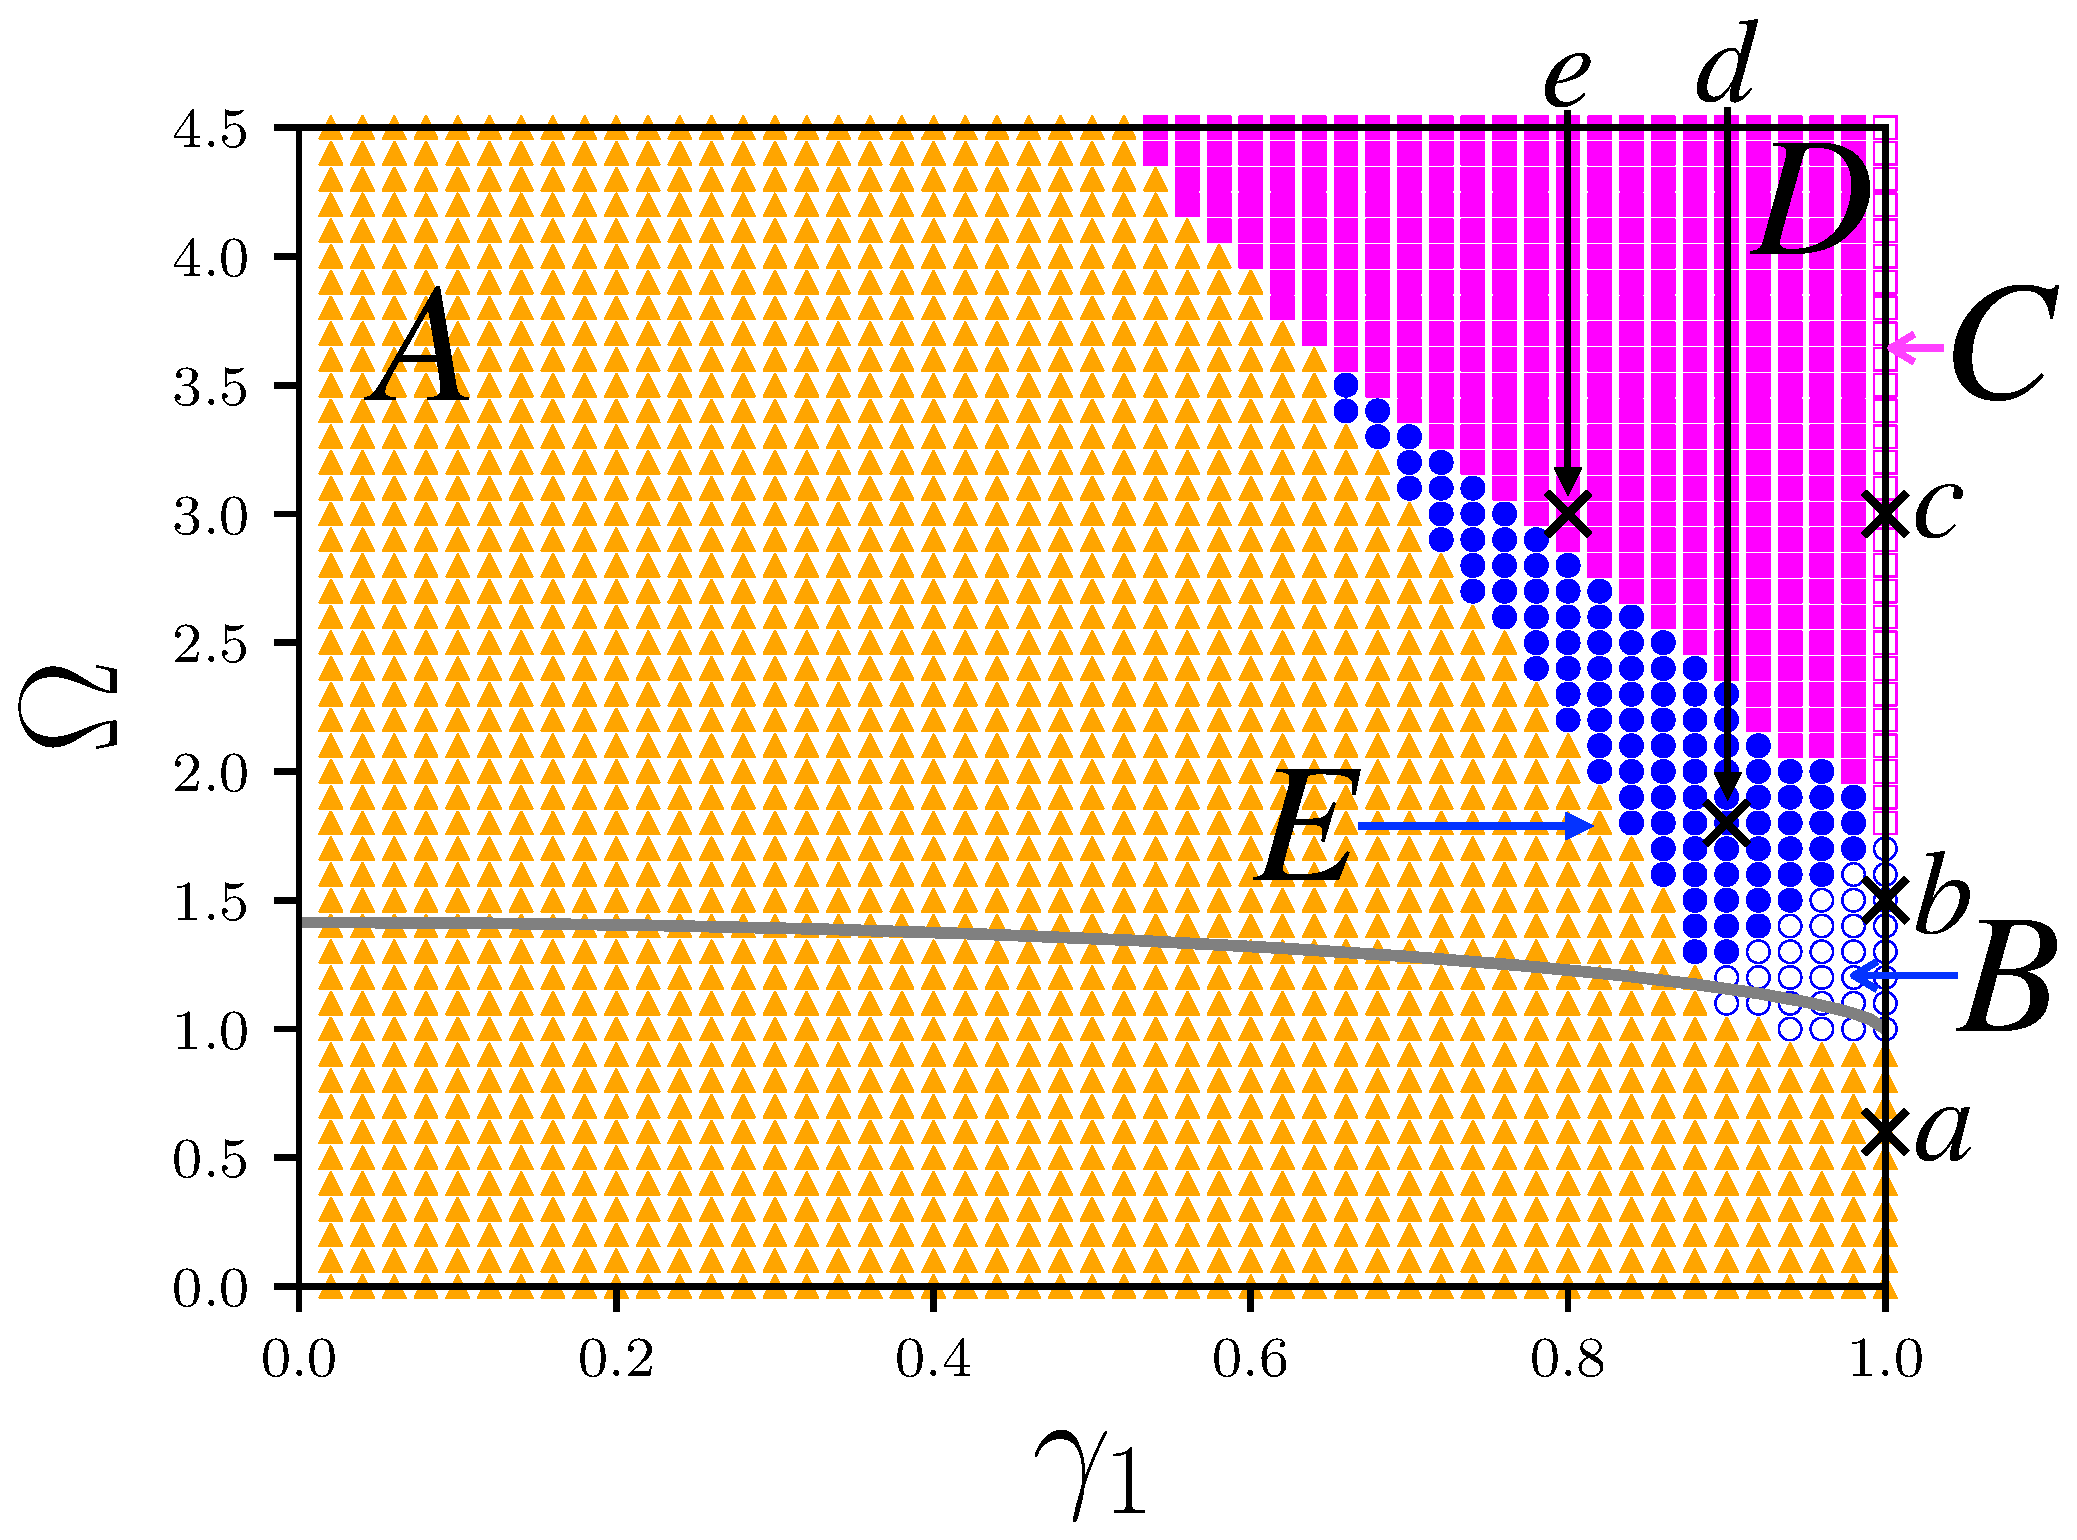
\includegraphics[width=8cm]{figs/pd-na.eps}
  \caption{Classification of the parameter plane
    ($\gamma_{1},\Omega$) into the five domains:
    A (filled orange triangles), B (open blue circles),
    C (open magenta squares),
    D (filled magenta squares), and E (filled blue circles).
    This classification is obtained by performing numerical simulations
    of the reduced system \eqref{eq:oa-12}.
    The gray line represents the borderline between
    the unimodal and bimodal natural frequency distributions $g(\omega)$.
    The bifurcation diagrams at the five points marked by the crosses
    are reported in Fig.~\ref{fig:bif-diagrams}.
    }
  \label{fig:phase-diagram}
\end{figure}


%%%%%%%%%%%%%%%%%%%%%%%%%%%%%%%%%%%%%%%%%%%
% For enlarging Fig.2
%\onecolumngrid
%%%%%%%%%%%%%%%%%%%%%%%%%%%%%%%%%%%%%%%%%%%

\begin{figure}
  \centering
  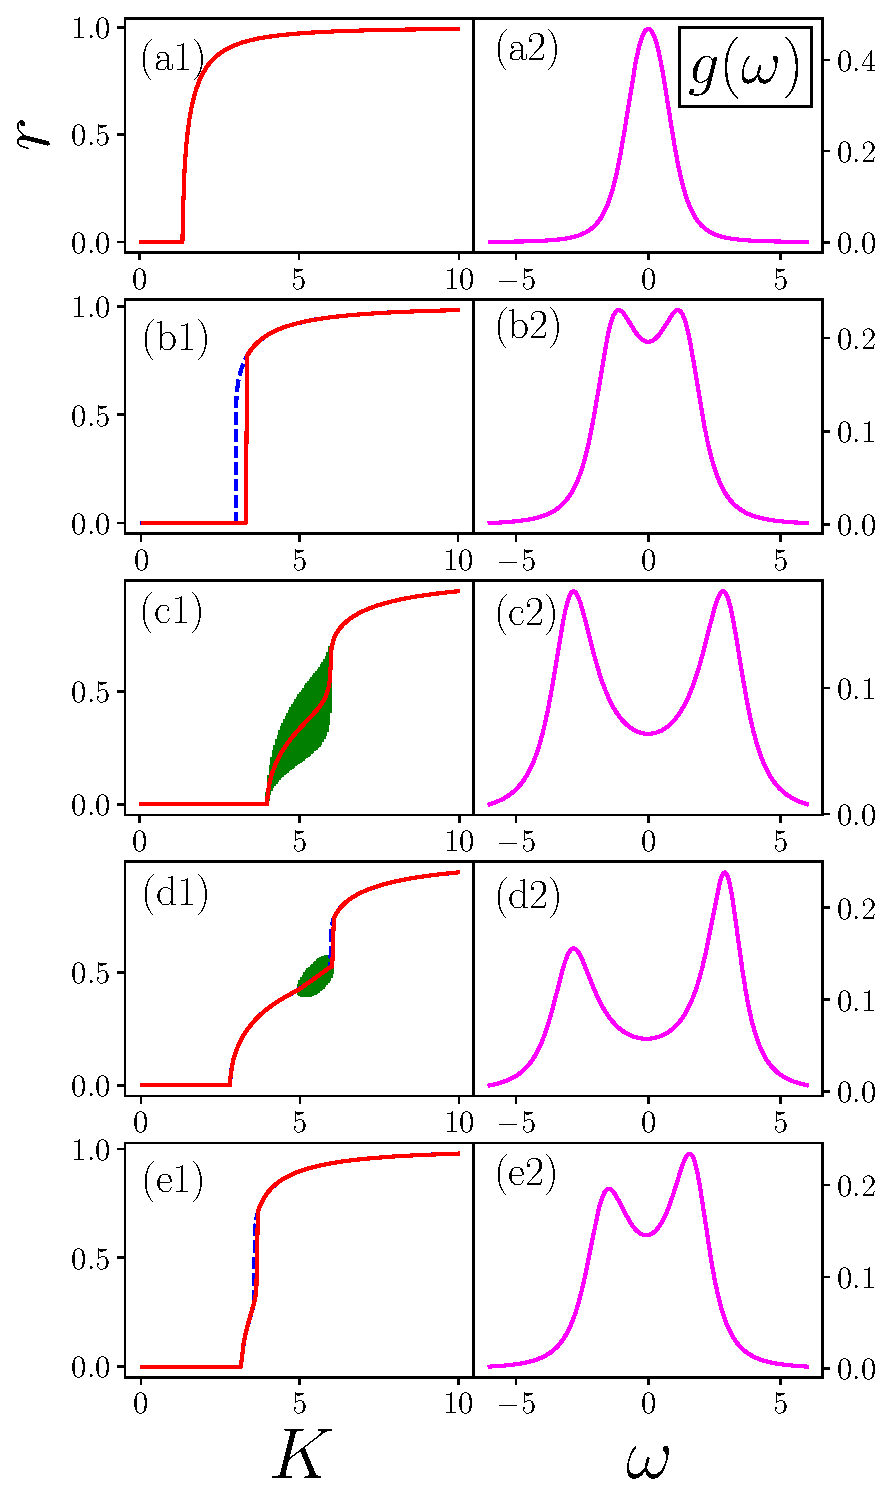
\includegraphics[width=8cm]{figs/bifurcation.eps}
  \caption{Five bifurcation diagrams at the five points
    marked on the parameter plane in Fig.~\ref{fig:phase-diagram}
    and the corresponding natural frequency distributions $g(\omega)$.
    The values of parameters $(\gamma_{1},\Omega)$ are
    (a) $(1.0,0.6)$, (b) $(1.0,1.5)$, (c) $(1.0,3.0)$,
    (d) $(0.8,3.0)$, and (e) $(0.9,1.8)$.
    In the panels (a1),(b1),(c1),(d1), and (e1),
    the red solid line and the blue dashed line
    respectively denote the forward
    and the backward process.
    In the panels (a1) and (c1), the backward process line
    collapses with the forward process line.
    Standard deviations of the order parameter
    are represented by the green vertical bars,
    but they are not visible in (a1), (b1), and (e1).
    The panels (a2),(b2),(c2),(d2), and (e2)
    show the natural frequency distributions
    $g(\omega)$ against $\omega$.
    }
  \label{fig:bif-diagrams}
\end{figure}

%%%%%%%%%%%%%%%%%%%%%%%%%%%%%%%%%%%%%%%%%%%
% End of onecolumngrid
%%%%%%%%%%%%%%%%%%%%%%%%%%%%%%%%%%%%%%%%%%%
%\twocolumngrid



\section{Theoretical analyses of equation of continuity}
\label{sec:analysis}

We shortly review linear and nonlinear analyses
of the equation of continuity \eqref{eq:kuramoto-inf}
around the nonsynchronized state $f^{0}$, which is explicitly written as
\begin{align}
  f^{0}(\omega) = \frac{g(\omega)}{2\pi}.
\end{align}
It is straightforward to check stationarity of $f^{0}$ as
\begin{align}
  \frac{\partial}{\partial\theta}(v[f^{0}]f^{0}) = 0
\end{align}
from the fact $v[f^{0}] = \omega$.
We expand the equation of continuity by substituting
\begin{align}
  F(\theta,\omega,t) = f^{0}(\omega) + f(\theta,\omega,t). 
\end{align}
The perturbation $f$ is governed by the equation
\begin{align}
  \frac{\partial f}{\partial t}=\mathcal{L}f+\mathcal{N}[f],
  \label{eq:expansion-f}
\end{align}
where the linear part is
\begin{align}
  \label{eq:linear-L}
  \mathcal{L}f
  = - \omega \dfrac{\partial f}{\partial\theta}
  - K f^{0} \dfrac{\partial}{\partial\theta}
  {\rm Im} \left( z(t) e^{-i\theta} \right)
\end{align}
and the nonlinear part is
\begin{align}
  \label{eq:nonlinear-N}
  \mathcal{N}[f]
  = - K \dfrac{\partial}{\partial\theta} \left[
    f~ {\rm Im}\left( z(t) e^{-i\theta} \right) \right]
\end{align}
with the order parameter
\begin{align}
  z(t) = \int_{-\infty}^{\infty} \diff\omega \int_{-\pi}^{\pi} \diff\theta
  e^{i\theta} f(\theta,\omega,t).
\end{align}
% \begin{align}
%   \mathcal{L}f
%   = -\omega \frac{\partial f}{\partial \theta}
%   + K f^{0} \frac{\partial}{\partial\theta} \int_{-\infty}^{\infty} ~\diff\omega'
%   \int_{-\pi}^{\pi} d\theta'~ \sin(\theta-\theta') f(\theta',\omega',t)
%   \label{eq:linear-L}
% \end{align}
% and the nonlinear part is
% \begin{align}
%   \mathcal{N}[f]
%   = K \frac{\partial}{\partial\theta} \left[
%     f \int_{-\infty}^{\infty} ~\diff\omega'
%     \int_{-\pi}^{\pi} d\theta'~ \sin(\theta-\theta') f(\theta',\omega',t)
%   \right].
% \end{align}
Note that the equation \eqref{eq:expansion-f} is an exact transform
from the equation of continuity \eqref{eq:kuramoto-inf}.
The linear part will be used to explain the oscillating state
emerging from a partially synchronized state
as well as a basic block of the amplitude equation.



\subsection{Linear analysis}
\label{eq:linear-eigenvalues}

The perturbation $f$ is a periodic function of $\theta$
and is expanded into the Fourier series as
\begin{align}
  f(\theta,\omega,t)
  = \sum_{k\in\mathbb{Z}} \widetilde{f}_{k}(\omega,t) e^{ik\theta}.
  \label{eq:f-Fourier}
\end{align}
The linear analysis of \eqref{eq:linear-L}
can be performed independently in each Fourier mode $k$
because the nonsynchronized state $f^{0}(\omega)$ does not depend on $\theta$.
The Fourier modes $k\neq \pm 1$ give only rotations,
and instability comes from the modes $k=\pm 1$.
The eigenvalues for the modes $k=\pm 1$ are obtained
as roots of the spectral functions
\begin{align}
  \Lambda_{\pm 1}(\lambda)
  = 1 - \frac{K}{2} \int_{-\infty}^{\infty}
  \frac{g(\omega)}{\lambda\pm i\omega} \diff\omega.
  \label{eq:spectral-function}
\end{align}
See Appendix \ref{sec:spectral-functions} for derivations.
If the real part of a root is positive, the eigenvalue induces instability.
We call such an eigenvalue as an unstable eigenvalue,
which is the target of the amplitude equation introduced
in the next subsection \ref{sec:amplitude-equation}.

We define the synchronization transition point $K_{\rm c}$
at which the nonsynchronized state $f^{0}$ changes stability.
This definition suggests that the eigenvalue having the largest real part
must be on the imaginary axis at $K_{\rm c}$.
A pure imaginary eigenvalue, however, induces a singularity
in the integrands of the spectral functions.
To avoid the singularity, we perform the analytic continuation
of $\Lambda_{\pm 1}(\lambda)$
and denote the continued functions as $D_{\pm 1}(\lambda)$.
See Appendix \ref{sec:analytic-continuation} for the continuation.


We give three remarks.
First, the continuation does not modify the spectral functions
in the region ${\rm Re}(\lambda)>0$,
and a root of $D_{\pm 1}(\lambda)$ whose real part is positive
is also a root of $\Lambda_{\pm 1}(\lambda)$.
Second, a root of $D_{\pm 1}(\lambda)$, however, may not be an eigenvalue
if it is on the region ${\rm Re}(\lambda)\leq 0$,
and the root is called a fake eigenvalue accordingly.
%Therefore, we do not need to introduce the term of unstable fake eigenvalue.
Third, the relations
\begin{align}
  \Lambda_{-1}(\lambda^{\ast}) = \Lambda_{1}^{\ast}(\lambda)
  \label{eq:relation-Lambda}
\end{align}
and 
\begin{align}
  D_{-1}(\lambda^{\ast}) = D_{1}^{\ast}(\lambda)
  \label{eq:relation-D}
\end{align}
hold, where $\Lambda_{1}^{\ast}(\lambda)$ is, for instance,
the complex conjugate of $\Lambda_{1}(\lambda)$.
%$=[\Lambda_{1}(\lambda)]^{\ast}$
% for instance and $[\Lambda_{1}(\lambda)]^{\ast}$ is the complex conjugate
% of $\Lambda_{1}(\lambda)$.
These relations imply that $\lambda^{\ast}$ is a (fake) eigenvalue
if $\lambda$ is.

For the family of natural frequency distributions \eqref{eq:g},
the equation $D_{1}(\lambda)=0$ leads a quadratic equation
of $\lambda$ and the two roots are denoted by $\lambda_{1}$ and $\lambda_{2}$
ordered as ${\rm Re}(\lambda_{1})\geq {\rm Re}(\lambda_{2})$.
In this paper, the two (fake) eigenvalues $\lambda_{1}$ and $\lambda_{2}$
are called the first and the second (fake) eigenvalues respectively.
See Appendix~\ref{sec:Kc} for the quadratic equation of $\lambda$,
the determination of the critical point $K_{\rm c}$,
and the number of unstable eigenvalues.


\subsection{Amplitude equation}
\label{sec:amplitude-equation}

We assume that the linear operator $\mathcal{L}$
has only one pair of unstable eigenvalues,
$\lambda_{1}$ and $\lambda_{1}^{\ast}$
coming from the relation \eqref{eq:relation-D},
and that the corresponding eigenfunctions are
$\Psi(\theta,\omega)$ and $\Psi^{\ast}(\theta,\omega)$ respectively.
To derive the amplitude equation, we expand $f$ into
\begin{align}
  f(\theta,\omega,t) = A(t) \Psi(\theta,\omega)
  + A^{\ast}(t) \Psi^{\ast}(\theta,\omega) + H(\theta,\omega, A, A^{\ast}).
  \label{eq:expand-f}
\end{align}
The amplitude $A$ relates to the order parameter $z$ as
\begin{align}
  z = 2\pi A^{\ast} + O(|A|^{3}),
\end{align}
and the asymptotic value of $z$ is approximately obtained by considering
temporal evolution of the amplitude $A(t)$.
The function $H$ represents the unstable manifold of
the nonsynchronized state $f^{0}$.
In other words, $H$ represents the height of the unstable manifold
from the eigenspace ${\rm Span}\{\Psi,\Psi^{\ast}\}$.
We assume that the unstable manifold is tangent
to the eigenspace ${\rm Span}\{\Psi,\Psi^{\ast}\}$
at $A=A^{\ast}=0$ and $H=O(|A|^{2})$ accordingly.

For deriving the amplitude equation,
we introduce the adjoint linear operator $\mathcal{L}^{\dagger}$ of $\mathcal{L}$
defined by
\begin{align}
  \left( \mathcal{L}^{\dagger} f_{1}, f_{2} \right)
  = \left( f_{1}, \mathcal{L} f_{2} \right),
  \quad
  \mathrm{ for }~\forall f_{1},f_{2},
\end{align}
where the inner product $(\cdot,\cdot)$ is defined by
\begin{align}
  \left( f_{1}, f_{2} \right)
  = \int_{-\infty}^{\infty} \diff\omega \int_{-\pi}^{\pi} \diff\theta
  f_{1}^{\ast}(\theta,\omega) ~ f_{2}(\theta,\omega).
\end{align}
Let $\widetilde{\Psi}$ and $\widetilde{\Psi}^{\ast}$
be the eigenfunctions of $\mathcal{L}^{\dagger}$
corresponding to the eigenvalues
$\lambda_{1}^{\ast}$ and $\lambda_{1}$ respectively.
We can choose the eigenfunctions satisfying the relations
\begin{align}
  \label{eq:normalization-tildePsi}
  \begin{aligned}
    & \left( \widetilde{\Psi}, \Psi \right) = 1,
     \quad
     \left( \widetilde{\Psi}, \Psi^{\ast} \right) = 0, \\
     & \left( \widetilde{\Psi}^{\ast}, \Psi \right) = 0,
     \quad
     \left( \widetilde{\Psi}^{\ast}, \Psi^{\ast} \right) = 1,
  \end{aligned}
\end{align}
without loss of generality. We also have
\begin{align}
  \left( \widetilde{\Psi}, H \right)
  = \left( \widetilde{\Psi}^{\ast}, H \right)
  = 0
  \label{eq:orthogonality-Psi-H}
\end{align}
because $H$ does not belong to the eigenspace ${\rm Span}\{\Psi,\Psi^{\ast}\}$.
See Appendix \ref{sec:adjoint} for the explicit expressions
of the adjoint operator and the eigenfunctions.

Substituting the expansion \eqref{eq:expand-f}
into the equation of continuity \eqref{eq:kuramoto-inf}
and using the relations \eqref{eq:normalization-tildePsi}
and \eqref{eq:orthogonality-Psi-H},
we have the amplitude equation as
\begin{align}
  \label{eq:amplitude-equation-general}
  \frac{{\rm d}A}{{\rm d}t}
  = \lambda_{1} A + \left( \widetilde{\Psi}, \mathcal{N}[f] \right)
\end{align}
and the equation for the unstable manifold $H$ as
\begin{align}
  \frac{{\rm d}H}{{\rm d}t}
  = \mathcal{L}H + \mathcal{N}[f]
  - \left[
    \left( \widetilde{\Psi}, \mathcal{N}[f] \right) \Psi
    + \left( \widetilde{\Psi}^{\ast}, \mathcal{N}[f] \right) \Psi^{\ast}
  \right].
  \label{eq:unstable-manifold-H}
\end{align}
These equations can be solved perturbatively for sufficiently small $|A|$,
and the right-hand-side of \eqref{eq:amplitude-equation-general}
is expanded as
\begin{align}
  \label{eq:amplitude-equation-complex}
  \frac{{\rm d}A}{{\rm d}t}
  = \lambda_{1} A + c_{3} A|A|^{2} + c_{5} A|A|^{4} + c_{7} A|A|^{6} + \cdots,
\end{align}
where the eigenvalue $\lambda_{1}$ and the coefficients $c_{3},c_{5},\cdots$
depend on the coupling constant $K$.
Note that the right-hand-side of \eqref{eq:amplitude-equation-complex}
has only odd order terms.
See Appendix \ref{sec:amp-eq} for derivations
and the explicit forms of coefficients.

The complex amplitude equation \eqref{eq:amplitude-equation-complex} can be
reduced to a real equation written as
\begin{align}
  \label{eq:amplitude-equation}
  \frac{{\rm d}\sigma}{{\rm d}t} = 2 \sigma G(\sigma),
\end{align}
where $\sigma=|A|^{2}\geq 0$ and
\begin{align}
  \label{eq:G-sigma}
  G(\sigma) = {\rm Re}(\lambda_{1}) + {\rm Re}(c_{3})\sigma
  + {\rm Re}(c_{5})\sigma^{2} + \cdots.
\end{align}
We will search for stationary solutions
with which the right-hand-side of the amplitude equation
\eqref{eq:amplitude-equation} is zero.
The nonsynchronized state,
for instance, corresponds to $\sigma=0$,
which always satisfies the stationary condition.

The amplitude equation is useful to determine
the continuity of the synchronization transition
from the nonsynchronized state $f^{0}$ 
to a partially synchronized state.
Around the critical point $K_{\rm c}$,
the order parameter must be small if the transition is continuous
and we can use the truncated equation
\begin{align}
  {\rm Re}(\lambda_{1}) + {\rm Re}(c_{3}) \sigma = 0.
\end{align}
%  Remembering the instability condition ${\rm Re}(\lambda_{1})>0$,
% For ${\rm Re}(c_{3})>0$, \red{on the contrary,}
% there is no solution of $\sigma\geq 0$ around the trivial one, $\sigma=0$,
  This equation has a nontrivial solution for ${\rm Re}(c_{3})<0$
  from the instability condition ${\rm Re}(\lambda_{1})>0$,
  while no real solution for ${\rm Re}(c_{3})>0$
  suggests a discontinuous transition.
Assuming continuity of $c_{3}(K)$ with respect to $K$
and taking the limit $K\to K_{\rm c}+0$, we say
that the synchronization transition is continuous
if ${\rm Re}(c_{3}(K_{\rm c}))<0$,
and is discontinuous if ${\rm Re}(c_{3}(K_{\rm c}))>0$ \cite{barre2016}.
%The separating point $\Omega=1$ on the symmetry line $\gamma_{1}=1$
%\red{
  The separating point $(\gamma_{1},\Omega)=(1,1)$
%}
between the domains A and B 
%\red{on the line $\gamma_{1}=1$}
on the line $\gamma_{1}=1$
is obtained by searching for
the point which satisfies ${\rm Re}(c_{3}(K_{\rm c}))=0$.




%%%%%%%%%%%%%%%%%%%%%%%%%%%%%%%%%%%%%%%%%%%%%%%%%%
% Reviced hereafter
%%%%%%%%%%%%%%%%%%%%%%%%%%%%%%%%%%%%%%%%%%%%%%%%%%

\section{Criteria for determining domains}
\label{sec:criteria}

Looking back the five bifurcation diagrams exhibited in Fig.~\ref{fig:bif-diagrams},
we have two elements to characterize the diagrams,
which are oscillation and a jump of the order parameter.
We first discuss mechanisms of the oscillation and of the jump
in Secs.~\ref{sec:oscillation} and \ref{sec:jump} respectively
with the aid of the linear and nonlinear analyses 
reviewed in the previous section \ref{sec:analysis}.
After that, we propose a procedure to divide the parameter plane
into the five domains in Sec.~\ref{sec:division}.

%We note that we are trying to capture the oscillation and the jump
%of the order parameter, which may be large enough for zero,
%by using a linear and a nonlinear analyses of the equation of continuity \ref{eq:kuramoto-inf}
%around the nonsynchronized state.

% \blue{
% In Sec.~\ref{sec:oscillation}, in order to observe the cluster
% formations, we perform $N$-body simulations of
% the Kuramoto model \eqref{eq:kuramoto}.
% As done in the reduced system, we use the fourth-order Runge-Kutta
% algorithm with the time step $\Delta t=0.01$.
% }

\subsection{Oscillation of order parameter}
\label{sec:oscillation}

%In this subsection, we deal with the oscillation of the order parameter.
The asymptotically periodic oscillation of the order parameter
has been also observed in the Hamiltonian mean-field model,
and the oscillation comes from existence of two small clusters
running with different velocities \cite{morita-kaneko-06}.
Inspired by this work, we propose the following idea;
The first unstable eigenvalue induces a partially synchronized state
and the oscillation is excited by appearance of a second unstable eigenvalue.

% We first discuss the oscillation of the order parameter
% by using the fake eigenvalues of the linear operator $\mathcal{L}$.
The order parameter is computed as
\begin{align}
  z(t)
  % = \int_{-\infty}^{\infty} ~\diff\omega \int_{-\pi}^{\pi} d\theta~
  % F(\theta,\omega,t) e^{i\theta}
  = 2\pi \int_{-\infty}^{\infty} \widetilde{f}_{-1}(\omega,t) \diff\omega,
\end{align}
the time evolution of the order parameter $z(t)$ is hence described
by the eigenvalues arisen from the Fourier $-1$ mode.
As defined in the end of Sec.~\ref{eq:linear-eigenvalues},
the two fake eigenvalues, the roots of $D_{-1}(\lambda)$,
are denoted by $\lambda_{1}^{\ast}$ and $\lambda_{2}^{\ast}$,
where ${\rm Re}(\lambda_{1}^{\ast})\geq{\rm Re}(\lambda_{2}^{\ast})$.


Let us increase the value of the coupling constant $K$
from the nonsynchronized region $K<K_{\rm c}$.
Beyond the critical point $K_{\rm c}$,
the first fake eigenvalue $\lambda_{1}^{\ast}$ becomes unstable
and the resonant oscillators,
whose natural frequencies are close to ${\rm Im}(\lambda_{1}^{\ast})$,
form a cluster.
For instance, if $g(\omega)$ is symmetric and unimodal,
the resonant frequency is zero
% because the unstable eigenvalue is zero,
% as discussed in Sec.~\ref{eq:linear-eigenvalues}.
% Consequently, 
and oscillators around $\omega=0$ form a synchronized cluster.
This small cluster corresponds to the continuous synchronization
transition in the bifurcation diagram (see Fig.~\ref{fig:bif-diagrams} (d)).
Further increasing $K$, for suitable pairs of $(\gamma_{1},\Omega)$,
the second fake eigenvalue $\lambda_{2}^{\ast}$ also becomes unstable
and forms the second cluster.
The two resonant frequencies differ in general,
${\rm Im}(\lambda_{1}^{\ast})\neq {\rm Im}(\lambda_{2}^{\ast})$,
and the order parameter oscillates;
The order parameter is large when the two clusters are close
on $\mathbb{S}^{1}$, and is small when the clusters are in the
antiphase positions each other.
The symmetry of $g(\omega)$, in particular, results
  in inducing simultaneous destabilization of the two fake
  eigenvalues $\lambda_{1}^{\ast}$ and $\lambda_{2}^{\ast}$ at $K_{\rm c}$
  and yielding the bifurcation diagram Fig.~\ref{fig:bif-diagrams} (c).
% that the two fake eigenvalues $\lambda_{1}^{\ast}$ and $\lambda_{2}^{\ast}$
% become unstable at $K_{\rm c}$.
% This simultaneous destabilization yields the bifurcation
% diagram Fig.~\ref{fig:bif-diagrams} (c).
% However, the symmetry does not always
% induce the simultaneous destabilization and only one
% fake eigenvalue gets unstable for $K>K_{\rm c}$,
% which yields the bifurcation diagrams Figs.~\ref{fig:bif-diagrams} (a) and (b).

Summarizing, existence of two unstable eigenvalues,
which mean two pairs of the unstable eigenvalues
by counting the roots of $D_{1}(\lambda)$ in addition to
the roots of $D_{-1}(\lambda)$,
suggests the oscillation of the order parameter.
To support this mechanism,
we investigate $K$ dependence of the fake eigenvalues
$\lambda_{1}^{\ast}$ and $\lambda_{2}^{\ast}$
at points chosen from the domains C, D, and E
of the parameter plane $(\gamma_{1},\Omega)$.


A symmetric case is examined in Fig.~\ref{fig:ev1030}
for $(\gamma_{1},\Omega)=(1.0,3.0)$ which belongs to the domain C.
As we expected, two eigenvalues become unstable
at the same $K_{\rm c}$ with different imaginary parts.
In Fig.~\ref{fig:phase-diagram}
the separating point $\Omega=\sqrt{3}$ between the domains B and C
on the symmetry line $\gamma_{1}=1$ is obtained
by checking existence of the two unstable eigenvalues.


\begin{figure}[htbp]
  \begin{center}
  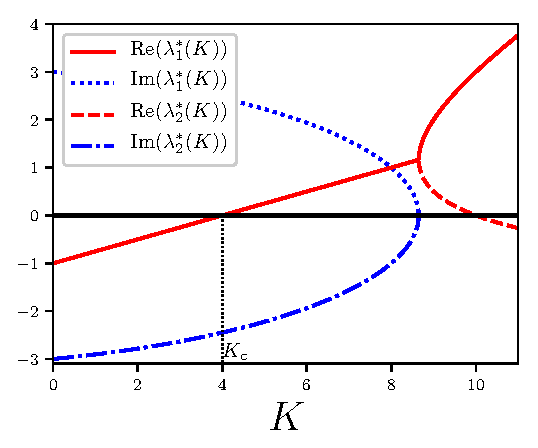
\includegraphics[width=8cm]{figs/ev1030.eps}  
  \end{center}
  \caption{$K$ dependence of the
    fake eigenvalues $\lambda_{1}^{\ast}$ and $\lambda_{2}^{\ast}$
    for $(\gamma_{1},\Omega)=(1.0,3.0)$.
    The lines representing
    $\mathrm{Re}(\lambda_{1}^{\ast}(K))$ (red solid line)
    and $\mathrm{Re}(\lambda_{2}^{\ast}(K))$ (red dashed line)
    collapse for $K\leq 4(\sqrt{10}-1)\simeq 8.649$.
    The two fake eigenvalues $\lambda_{1}^{\ast}$ and $\lambda_{2}^{\ast}$
    become unstable simultaneously at $K_{\rm c}=4$.
  }
  \label{fig:ev1030}
\end{figure}


For the point $(\gamma_{1},\Omega)=(0.8,3.0)$
belonging to the domain D, 
the simultaneity of destabilization
breaks as shown in Fig.~\ref{fig:ev0830}
owing to asymmetry of $g(\omega)$.
A correspondence between the two unstable
eigenvalues and the two clusters is exhibited in Fig.~\ref{fig:cluster1},
where $N$-body simulations of the Kuramoto model \eqref{eq:kuramoto}
were performed by using the fourth-order Runge-Kutta algorithm
with the time step $\Delta t=0.01$.
See Appendix \ref{sec:capture_cluster}
  for the procedure to determine the synchronized intervals of $\omega$
  reported as red bars in Fig.~\ref{fig:cluster1}.
% The emergence of the second cluster 
% in good agreement with the emergence of the second unstable eigenvalue
% even when the point $(\gamma_{1},\Omega)$ is
% far from the domain C.
%See Fig.~\ref{fig:cluster3} for the point $(\gamma_{1},\Omega)=(0.6,4.0)$.
% To the contrary, at the point $(\gamma_{1},\Omega)=(0.9,1.8)$ 
% belonging to the domain E but close to the domain D,
% the second fake eigenvalue approaches to zero but does not become unstable
% as reported in Fig.~\ref{fig:ev0918}.
The second unstable eigenvalue and the second cluster emerge
  at almost same values of $K$,
  and this observation is consistent with the discussion above.
  The scenario holds even when the first cluster is further developed
  as shown in Fig.~\ref{fig:cluster3} for the point $(\gamma_{1},\Omega)=(0.6,4.0)$,
  although the linear analysis is performed around the
  nonsynchronized state.
  It is worth noting that the second fake eigenvalue approaches
  to zero but does not become unstable
  at the point $(\gamma_{1},\Omega)=(0.9,1.8)$
  close to the domain D but belonging to the domain E
  as reported in Fig.~\ref{fig:ev0918}.


\begin{figure}[htbp]
  \begin{center}  
  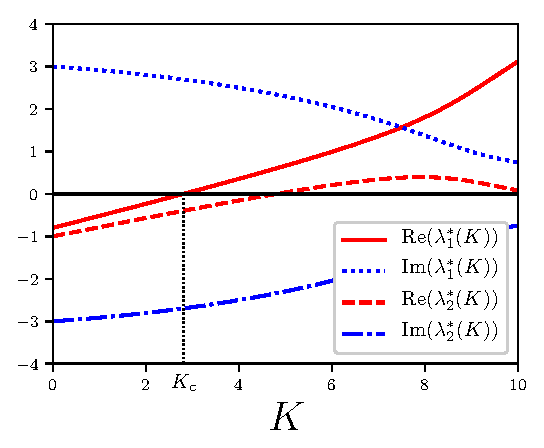
\includegraphics[width=8cm]{figs/ev0830.eps}
  \end{center}
  \caption{$K$ dependence of the
    fake eigenvalues $\lambda_{1}^{\ast}$ and $\lambda_{2}^{\ast}$
    for $(\gamma_{1},\Omega)=(0.8,3.0)$ belonging to the domain D.
    The first fake eigenvalue $\lambda^{\ast}_{1}$ becomes unstable
    at the critical point $K_{\rm c}=2.807$,
    then the second fake eigenvalue $\lambda^{\ast}_{2}$ becomes
    unstable at a larger $K=4.794$.
  }
  \label{fig:ev0830}
\end{figure}

\begin{figure}[htbp]
\begin{center}
  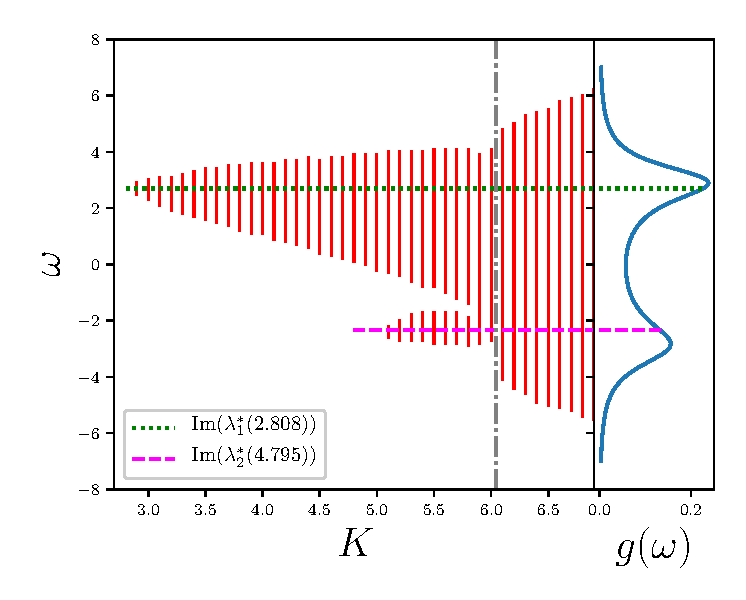
\includegraphics[width=8cm]{figs/cluster1.eps}
\end{center}
  \caption{
    The natural frequency distribution and the emerging clusters
    for $(\gamma_{1},\Omega)=(0.8,3.0)$.
    The clusters, which are obtained by numerically integrating
    the $N$-body system \eqref{eq:kuramoto} with $N=10^{5}$,
    are found in the ranges of red bars.
    The second fake eigenvalue $\lambda_{2}^{\ast}$
    becomes unstable at $K=4.795$,
    which is approximately in agreement with the emergence point of the second lower cluster.
    %\red{
      Merging two clusters occurs around $K=6.04$, which is 
      plotted with gray dash-dotted line,
      and this leads to the jump in the order parameter,
      as seen in Fig.~\ref{fig:bif-diagrams}(d1).
    %}
  }
  \label{fig:cluster1}
\end{figure}

\begin{figure}[htbp]
\begin{center}
  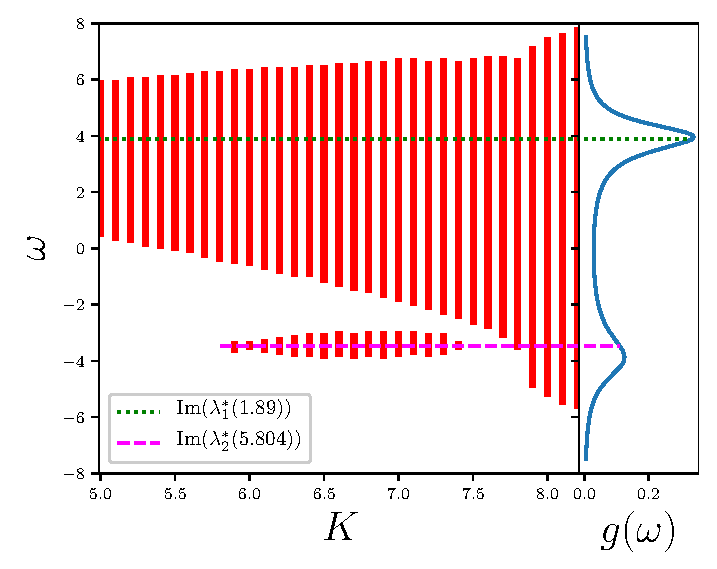
\includegraphics[width=8cm]{figs/cluster3.eps}
\end{center}
  \caption{
    Same with Fig.~\ref{fig:cluster1} but for $(\gamma_{1},\Omega)=(0.6,4.0)$
    belonging to the domain D.
    The second fake eigenvalue $\lambda_{2}^{\ast}$
    becomes unstable at $K=5.804$,
    which is approximately in agreement with the emergence point of the second lower cluster.
    The second cluster does not merge
    into the first cluster,
    and the the second cluster vanishes around
    $K=7.5$.
    }
  \label{fig:cluster3}
\end{figure}

\begin{figure}[htbp]
\begin{center}
  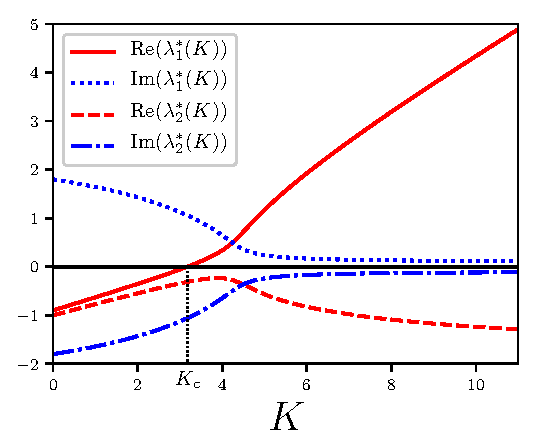
\includegraphics[width=8cm]{figs/ev0918.eps}
\end{center}
  \caption{Same with Fig.~\ref{fig:ev0830}
    but for $(\gamma_{1},\Omega)=(0.9,1.8)$ belonging to the domain E.
    The real part of the fake eigenvalue $\lambda_{2}$ approaches to zero,
    but does not become positive.}
  %Kc=3.17622335
  \label{fig:ev0918}
\end{figure}


We note that the discussion above does not always hold
because the second unstable eigenvalue
does not always yield the second cluster.
At the point $(\gamma_{1},\Omega)=(0.8,2.6)$ belonging to the domain E,
at $K=5.032$, the second unstable eigenvalue emerges
but its imaginary part is not sufficiently far from
the grown first cluster,
and the second virtual cluster is absorbed by the first cluster
without emerging as shown in Fig.~\ref{fig:cluster2}.
One more condition must be therefore added to characterize the oscillation;
%$|{\rm Im}(\lambda_{1}^{\ast})-{\rm Im}(\lambda_{2}^{\ast})|$
%must be sufficiently large \cite{barre-yamaguchi-09}.
%\red{
\begin{align}
  |{\rm Im}(\lambda_{1}^{\ast})-{\rm Im}(\lambda_{2}^{\ast})|>s
  \label{eq:imag-condition}
\end{align}
for some $s$ \cite{barre-yamaguchi-09}.
%It is not straightforward to determine the threshold
%for this discrepancy and we leave this condition as a future problem.
See Appendix~\ref{sec:imag-condition} for the further investigation on this condition.
%}

\begin{figure}[htbp]
\begin{center}
  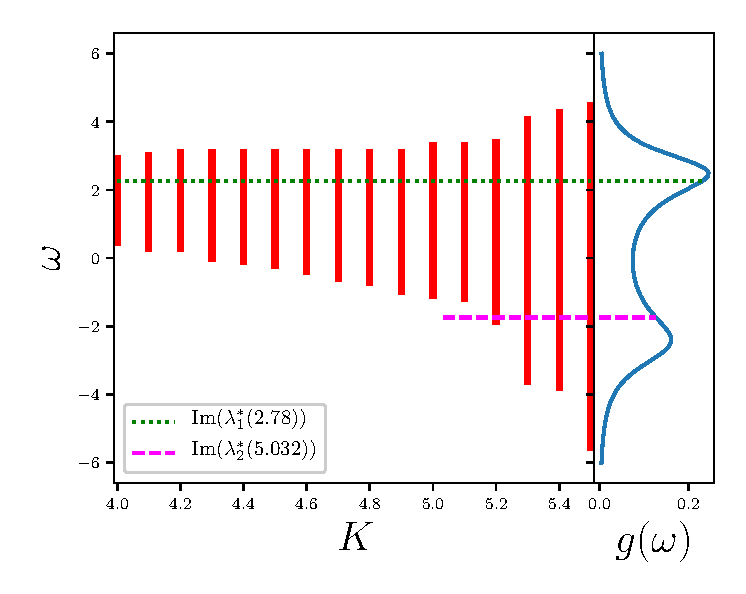
\includegraphics[width=8cm]{figs/cluster2.eps}
\end{center}
  \caption{
  %   The cluster formed at $(\gamma_{1},\Omega)=(0.8,2.6$)
  % and the corresponding natural frequency distribution.
  % The red lines denote the $\omega$-range of the cluster 
  % formed at $K$ between $[4.0,5.5]$.
  % The first eigenvalue $\lambda_{1}$ becomes unstable at $K_{\rm c}=2.78039554$
  % and the second eigenvalue $\lambda_{2}$ becomes unstable at $K=5.03248799$.
  % We see that the second cluster
  % did not show up through increasing $K$,
  % though the second unstable eigenvalue $\lambda_{2}$ emerges.
  % We note that this cluster is obtained
  % by numerically integrating the $N$-body system
  % Eq.~\ref{eq:kuramoto} with $(\gamma_{1},\Omega)=(0.8,2.6)$
  % and $K\in[4.0,5.5]$
  % ($N=10^{5}$).
    %
    Same with Fig.~\ref{fig:cluster1} but for $(\gamma_{1},\Omega)=(0.8,2.6)$
    belonging to the domain E.
    The second fake eigenvalue becomes unstable at $K=5.032$,
    but the second cluster does not appear.}
  \label{fig:cluster2}
\end{figure}

% Interestingly,
% we find that for some points in $(\gamma_{1},\Omega)$,
% more than two clusters emerges for some $K$.
% These states are called Bellerophon states,
% as reported in \cite{bi2016,li2019}. 
% Fig.~\ref{fig:cluster5} shows the emerging clusters
% for $(\gamma_{1},\Omega)=(0.82,4.5)$.
% %The first cluster emerges at $K_{\mathrm{c}}\sim 2.96$.
% %Then the second cluster,
% %corresponding to the second unstable eigenvalue,
% %emerges around $K\sim 4.52$.
% %As $K$ further increases,
% %two more clusters emerge from positive and negative
% %frequencies around $K\sim 6.8$,
% %and another two clusters emerge around $K\sim 7.5$
% Past researches on the Bellerophon states
% were focusing on the symmetric frequency distributions.
% We have found that the Bellerophon states can be found
% also on the asymmetric frequency distributions.

  We give another remark on multi-cluster states;
  The maximum number of clusters is not necessarily two
  for the bimodal natural frequency distribution.
  Multi-cluster states called the Bellerophon states
  are reported in \cite{bi2016,li2019}
  for symmetric natural frequency distributions.
  The symmetry is, however, not essential to the multi-cluster states
  as an example is shown in Fig.~\ref{fig:cluster5}
  for an asymmetric distribution with $(\gamma_{1},\Omega)=(0.82,4.5)$.


\begin{figure}[htbp]
\begin{center}
  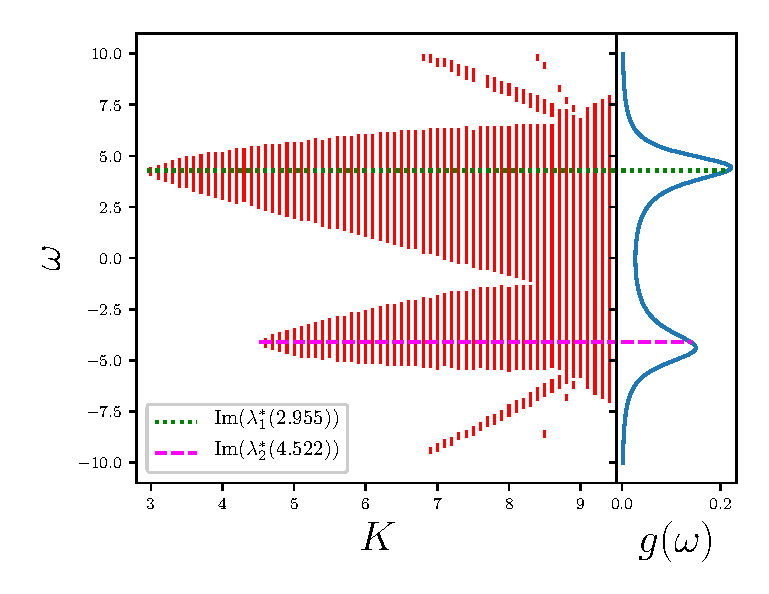
\includegraphics[width=8cm]{figs/cluster5.eps}
\end{center}
  \caption{
    Same with Fig.~\ref{fig:cluster1} but for $(\gamma_{1},\Omega)=(0.82,4.5)$
    belonging to the domain E.
    The second fake eigenvalue $\lambda_{2}^{\ast}$
    becomes unstable at $K=4.522$,
    which is approximately in agreement with the emergence point of the second lower cluster.
    There exists clusters
    other than the first and second clusters corresponding
      to the two peaks of the natural frequency distribution $g(\omega)$.
    This multi-cluster state is referred to as the Bellerophon state \cite{bi2016,li2019}.}
  \label{fig:cluster5}
\end{figure}



\subsection{Jump of order parameter}
\label{sec:jump}

A jump of the order parameter emerges from $r=0$ (domain B)
or from $r>0$ (domain E) .
We expect that the jump from $r=0$ is identified
by ${\rm Re}(c_{3}(K_{\rm c}))>0$
as discussed in Sec.~\ref{sec:amplitude-equation}.
This criterion is successfully used in a generalized model \cite{barre2016},
but for symmetric natural frequency distributions.
We will verify this criterion for asymmetric ones with $\gamma<1$.

To characterize the jump from $r>0$,
a typical bifurcation diagram of the type E is schematically shown
in Fig.~\ref{fig:schematic2}.
We focus on the saddle-node bifurcation point $K_{\rm Q}$,
at which $G(\sigma)$ in the amplitude equation \eqref{eq:amplitude-equation}
has degenerated nontrivial roots.
The degeneracy can be approximately captured by $G_{2}(\sigma)$,
the truncation of $G(\sigma)$ up to the second order of $\sigma$,
as the vanishing discriminant.

Let us discuss validity of the expansion \eqref{eq:amplitude-equation-complex}
around the saddle-node bifurcation point $K_{\rm Q}$.
The point $K_{\rm Q}$ is approximated by $K_{\rm Q'}$ obtained from $G_{2}(\sigma)$.
The value of $\sigma$ at $K_{\rm Q}$ is also approximated as
\begin{align}
  \sigma_{\ast}' = - \dfrac{{\rm Re}(c_{3}(K_{\rm Q'}))}{{\rm Re}(c_{5}(K_{\rm Q'}))}
\end{align}
and gives the equality
\begin{align}
  \label{eq:ratio-35}
  \dfrac{|{\rm Re}(c_{5}(K_{\rm Q'}))(\sigma_{\ast}')^{2}|}
  {|{\rm Re}(c_{3}(K_{\rm Q'}))\sigma_{\ast}'|} = \dfrac{1}{2}.
\end{align}
This equality suggests that the expansion \eqref{eq:amplitude-equation-complex}
up to the third term is not excellent but
does not break around the bifurcation point $K_{\rm Q}$.
We will discuss validity of \eqref{eq:amplitude-equation-complex} later
from the view point of smallness of the order parameter.

We remark on the upper stable branch appearing
at another saddle-node bifurcation point $K_{\rm P}$.
Coexistence of the three branches between $K_{\rm P}$ and $K_{\rm Q}$
is a distinguishing feature of the type E,
%Focusing on $K_{\rm Q}$, \red{however,} has two advantages:
but we focus on $K_{\rm Q}$ because of the two advantages:
(i) Capturing the coexistence in the amplitude equation
\eqref{eq:amplitude-equation} requires the third order term of $G(\sigma)$,
the coefficient $c_{7}$, which is hard to compute.
(ii) The upper branch has a larger value of $\sigma$ than $\sigma_{\ast}'$,
and validity of the expansion \eqref{eq:amplitude-equation-complex}
becomes worse accordingly.


\begin{figure}[htbp]
\begin{center}
  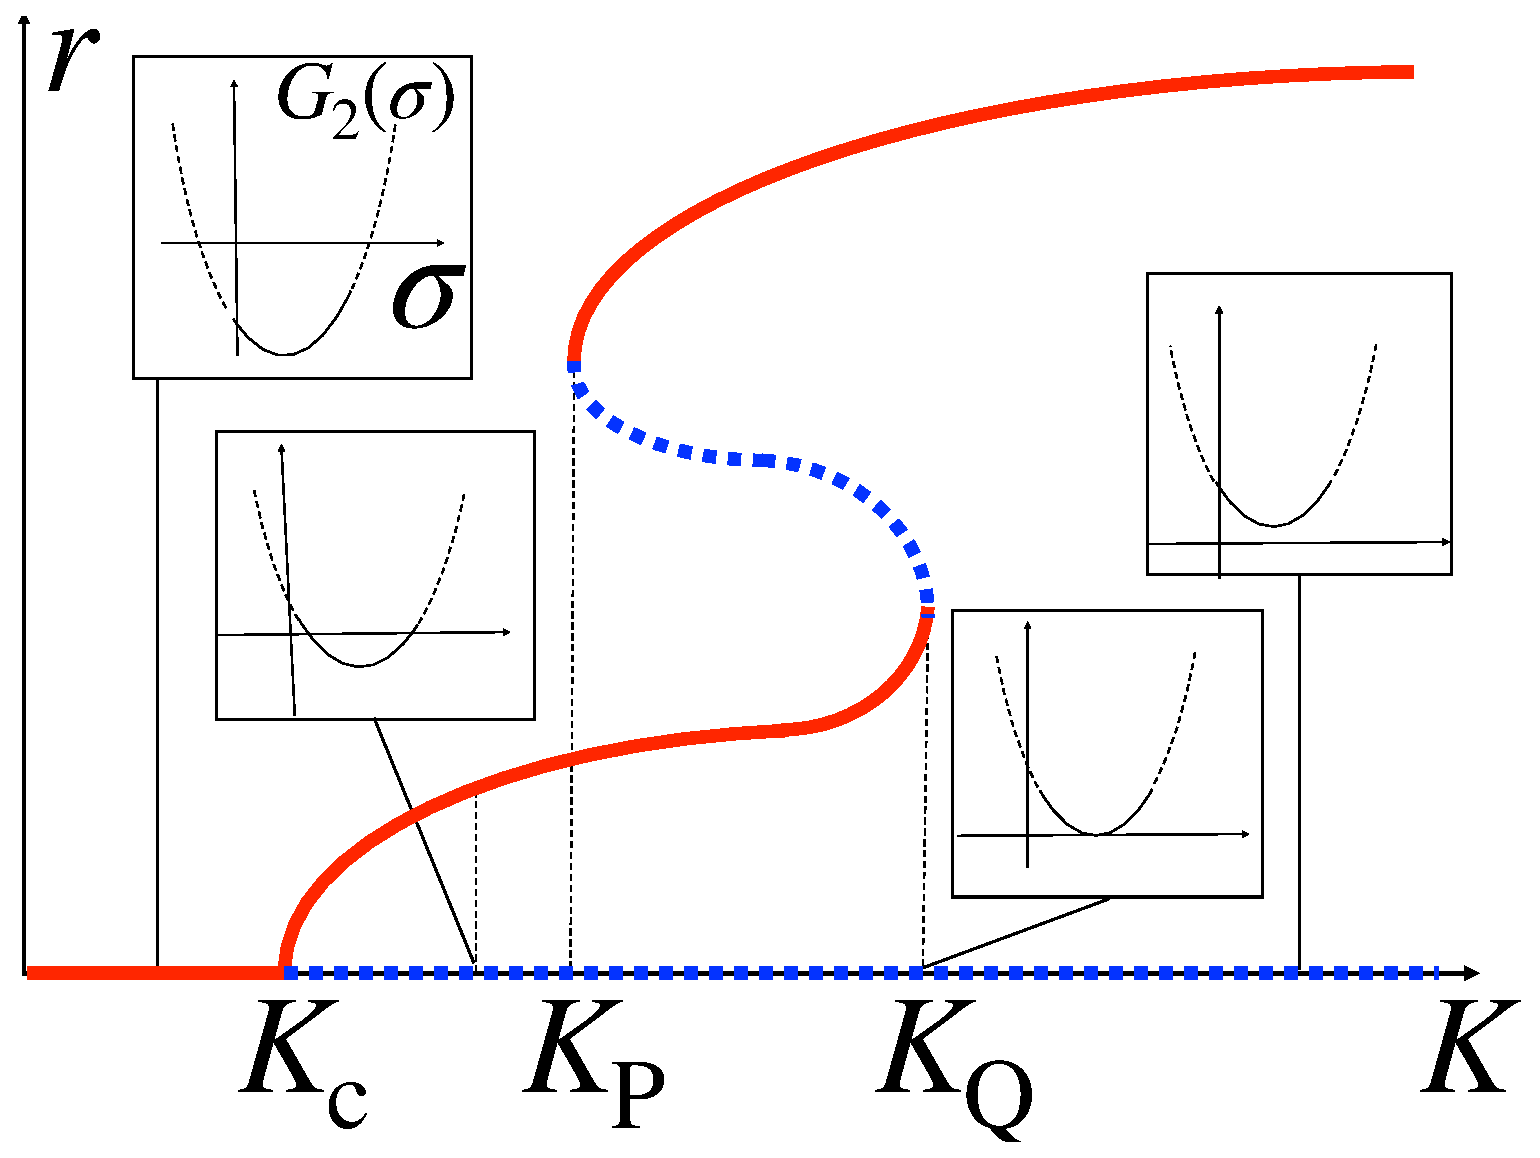
\includegraphics[width=8cm]{figs/G2_sigma.eps}
\end{center}
\caption{
  Schematic picture for the bifurcation diagram of type E.
  The red solid lines denote the stable branches,
  and the blue dashed lines denote the unstable branches.
  Insets are schematic graphs of $G_{2}(\sigma)$.  
  }
  \label{fig:schematic2}
\end{figure}


% These nontrivial values of $r$ correspond to nontrivial positive
% roots of $G(\sigma)$ in the amplitude equation \eqref{eq:G-sigma}.
% To capture the three nontrivial roots of the type E,
% we consider $G(\sigma)$ up to the third order,
% which is denoted by $G_{3}(\sigma)$.
% Corresponding to the four values of $K_{i}~(i=1,2,3,4)$
% in Fig. \ref{fig:schematic2},
% four schematic graphs of $G_{3}(\sigma)$ are shown
% in Fig.~\ref{fig:schematic1}.
% Existence of three roots is expressed by the positive discriminant
% of $G_{3}(\sigma)$.
% However, this criterion fails to identify the domain E.
% The amplitude equation is derived by using a perturbation technique
% and validity for a large amplitude, like the upper stable branch
% in Fig. \ref{fig:schematic2}, is not guaranteed.
% We, therefore, change the strategy.

% We focus on the bifurcation point $K_{\rm Q}$,
% which characterizes the type E.
% The point $K_{\rm Q}$ is approximated by $K_{\rm Q'}$,
% which is obtained from $G_{2}(\sigma)$,
% the truncation of $G(\sigma)$ up to the second order.
% The value of $\sigma$ at $K_{\rm Q'}$ is also approximated as
% \begin{align}
%   \sigma_{\ast}' = - \dfrac{{\rm Re}(c_{3}(K_{\rm Q'}))}{{\rm Re}(c_{5}(K_{\rm Q'}))}
% \end{align}
% and gives the equality
% \begin{align}
%   \dfrac{|{\rm Re}(c_{5}(K_{\rm Q'}))(\sigma_{\ast}')^{2}|}
%   {|{\rm Re}(c_{3}(K_{\rm Q'}))\sigma_{\ast}'|} = \dfrac{1}{2}.
% \end{align}
% This equality suggests that
% the expansion \eqref{eq:amplitude-equation-complex}
% does not break at the bifurcation point $K_{\rm Q}$
% and that we can capture existence of $K_{\rm Q}$
% through degeneracy of the roots of $G_{2}(\sigma)$.

%To ensure the validity of perturbation, we require the condition
% \begin{align}
%   \left| \mathrm{Re}(c_{3}(K))\sigma \right|
%   \gg \left| \mathrm{Re}(c_{5}(K))\sigma^{2} \right|
%   \gg \left| \mathrm{Re}(c_{7}(K))\sigma^{3} \right|.
%   \label{eq:per-cond-text}
% \end{align}
% However, Setting $\sigma$ which corresponds to the value $r(K_{Q})$,
% the condition breaks almost any point on the parameter plane
% $(\gamma_{1},\Omega)$ due to the third order term,
% while the first and second order terms satisfy
% \begin{align}
%   \left| \mathrm{Re}(c_{3}(K))\sigma \right|
%   = 2 \left| \mathrm{Re}(c_{5}(K))\sigma^{2} \right|.
% \end{align}
% See Appendix~\ref{sec:c7}.
% The largest $r$ among the three nontrivial solutions
% at $K_{3}$ may break validity of the perturbation,
% even the other two nontrivial solutions are sufficiently small.
% This breaking happens actually 
% and is discussed in Appendix~\ref{sec:c7}.


% We, therefore, change the strategy as follows.
% At least around the domain B,
% we may expect that the continuous transition branch,
% the lower nontrivial stable branch in Fig.~\ref{fig:schematic2},
% should be short and that the bifurcation point at $K_{Q}$
% is close to $r=0$.
% This bifurcation point is captured by truncating $G(\sigma)$
% up to the second order, denoted by $G_{2}(\sigma)$.
% Thus, the new criterion to characterized the domain E is that
% there exists $K>K_{\rm c}$ at which
% the discriminant of $G_{2}(\sigma)$ is zero.



\subsection{Theoretical division of the parameter plane}
\label{sec:division}

In the basis of the discussions done in Secs.~\ref{sec:oscillation} and \ref{sec:jump},
we divide the parameter plane $(\gamma_{1},\Omega)$
into the five domains by the following flow.
For preparation, we compute the critical point $K_{\rm c}$
for a given pair of parameters $(\gamma_{1},\Omega)$
as shown in Appendix \ref{sec:Kc}.

We first focus on the critical point $K=K_{\rm c}$.
The discontinuous jump appears at $K_{\rm c}$ only in the type B
among the considered five bifurcation diagrams
(see Fig.~\ref{fig:bif-diagrams}).
The point $(\gamma_{1},\Omega)$ must belong to the domain B
if ${\rm Re}(c_{3}(K_{\rm c}))>0$ holds, which suggests a jump from $r=0$.
When this condition does not hold,
we check if there are two unstable eigenvalues at $K_{\rm c}$.
If this condition is satisfied, oscillation of the order parameter
starts from $K_{\rm c}$ and the point $(\gamma_{1},\Omega)$
is considered to be in the domain C.

When both checks at $K_{\rm c}$ are negative, 
we increase $K$ from $K_{\rm c}$ and examine the following two propositions:
\begin{align}
  \mathrm{(Oscillation) }\ 
  \exists K_{\rm O} (>K_{\rm c})\ 
  \mathrm{ s.t. }\ 
  {\rm Re}(\lambda_{2}(K_{\rm O}))>0,
  \label{eq:proposition-oscillation}
\end{align}
and
\begin{align}
  \mathrm{(Jump) }\ 
  \exists K_{\rm J} (>K_{\rm c})\ 
  \mathrm{ s.t. }\ 
  %\blue{\Delta(K_{2}) = 0},
  \Delta(K_{\rm J}) = 0,
  \label{eq:proposition-jump}
\end{align}
where the discriminant $\Delta(K)$ of $G_{2}(\sigma)$ is defined by
\begin{align}
  \Delta(K)
  = {\rm Re}(c_{3}(K))^{2} - 4{\rm Re}(\lambda(K)){\rm Re}(c_{5}(K)).
\end{align}
Note that the degenerated root of $G_{2}(\sigma)$, $-c_{3}/(2c_{5})$,
is positive under the assumptions $c_{3}(K_{\rm J})<0$ and $c_{5}(K_{\rm J})>0$.
If both the propositions \eqref{eq:proposition-oscillation}
and \eqref{eq:proposition-jump} are false, we decide that the point
$(\gamma_{1},\Omega)$ belongs to the domain A.
If the oscillation proposition \eqref{eq:proposition-oscillation}
is true but the jump proposition \eqref{eq:proposition-jump} is false,
the point must be in the domain D.
If the oscillation proposition \eqref{eq:proposition-oscillation}
is false but the jump proposition \eqref{eq:proposition-jump} is true,
the point must be in the domain E.
If both the propositions are true, there is a competition
between $K_{\rm O}$ and $K_{\rm J}$; $K_{\rm O}<K_{\rm J}$ suggests the domain D
and $K_{\rm O}>K_{\rm J}$ suggests the domain E.
% \red{
%   We summarize what techniques we use to determine each domain in Table~\ref{table:tech-domain}.
% }
%\red{
  In Table~\ref{table:tech-domain}, 
  we summarize techniques which are used to determine the domains
%  }

%\begin{table}
%  \caption{The techniques we use to determine the domains.}
%  \label{table:tech-domain}
%  \begin{tabular}{c||ccccc}
%   & 
%   \begin{minipage}{10mm}
%     \scalebox{0.2}{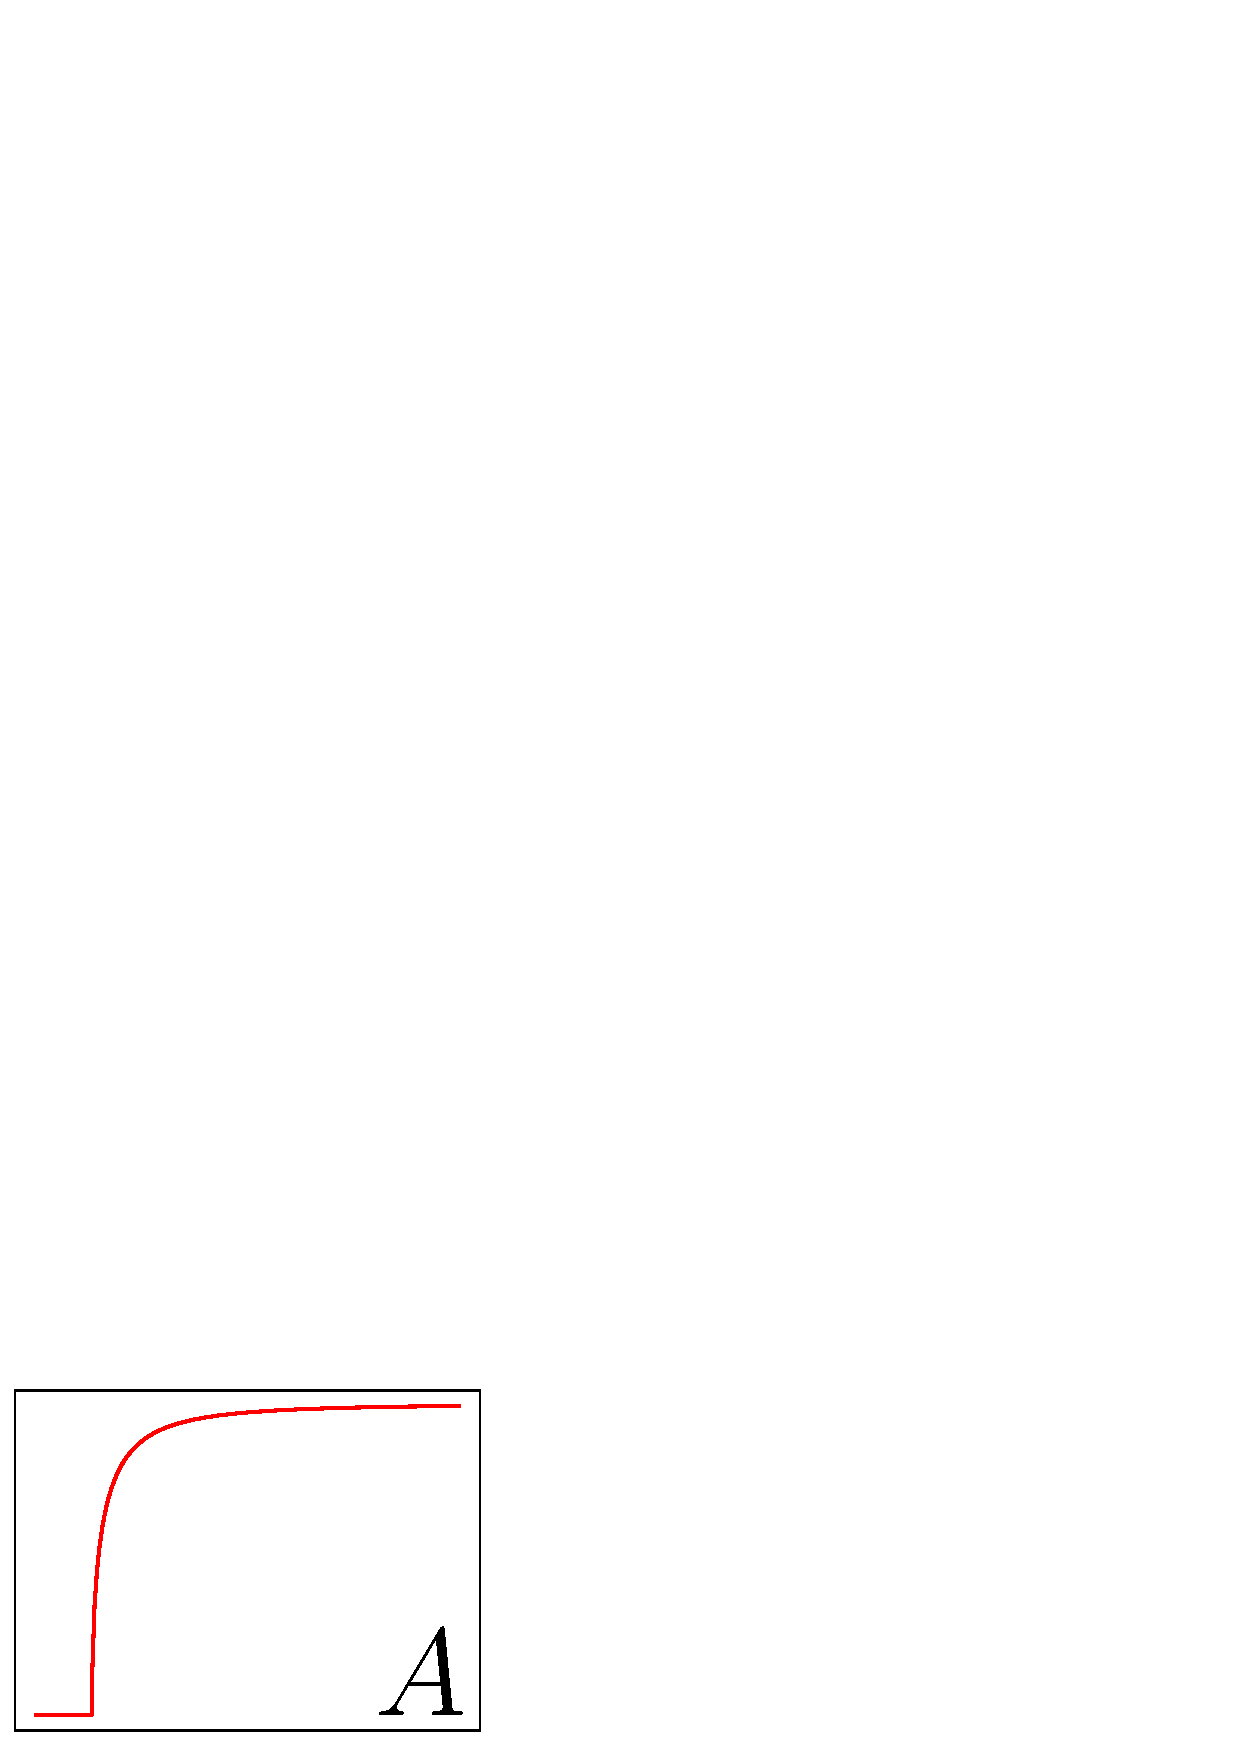
\includegraphics{A.pdf}}
%   \end{minipage}
%   & 
%   \begin{minipage}{10mm}
%    \scalebox{0.2}{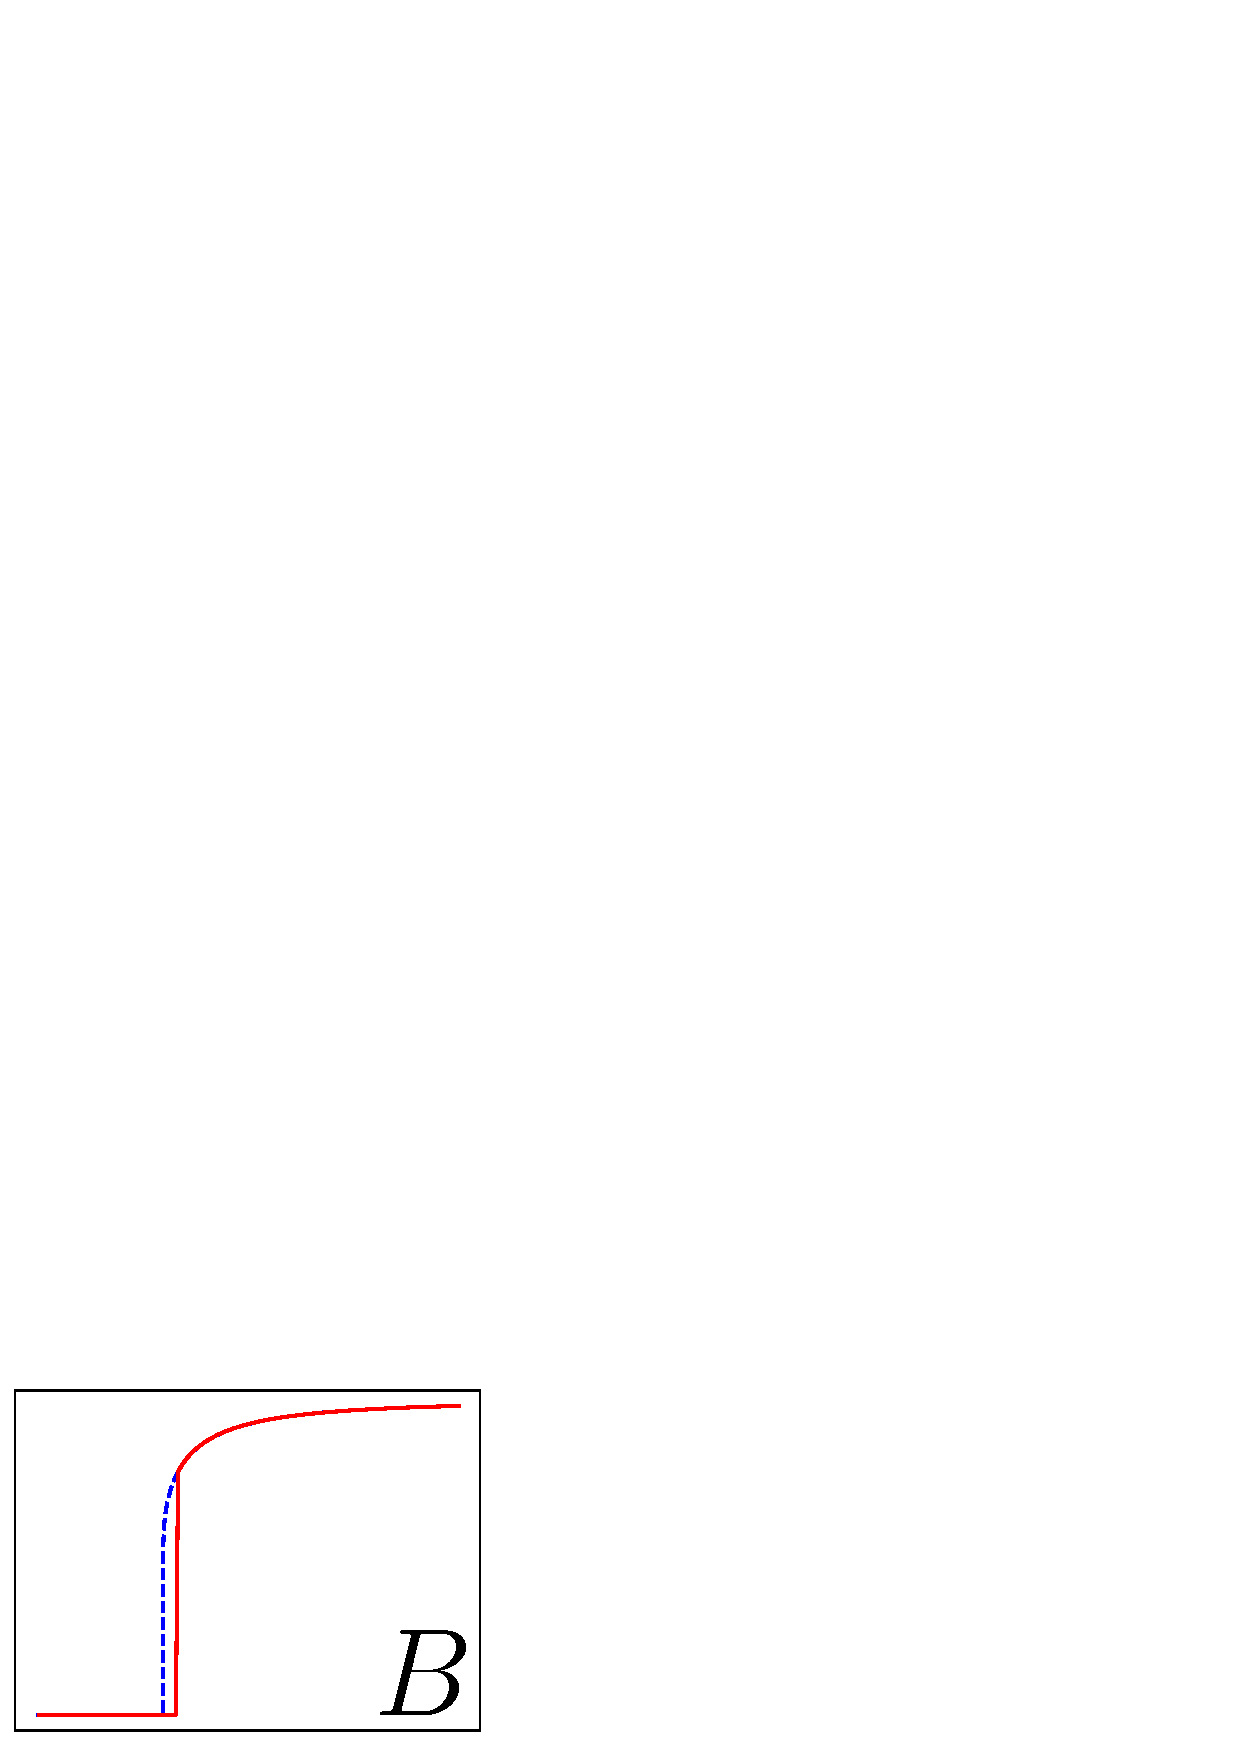
\includegraphics{B.pdf}}
%  \end{minipage}
%   & 
%   \begin{minipage}{10mm}
%    \scalebox{0.2}{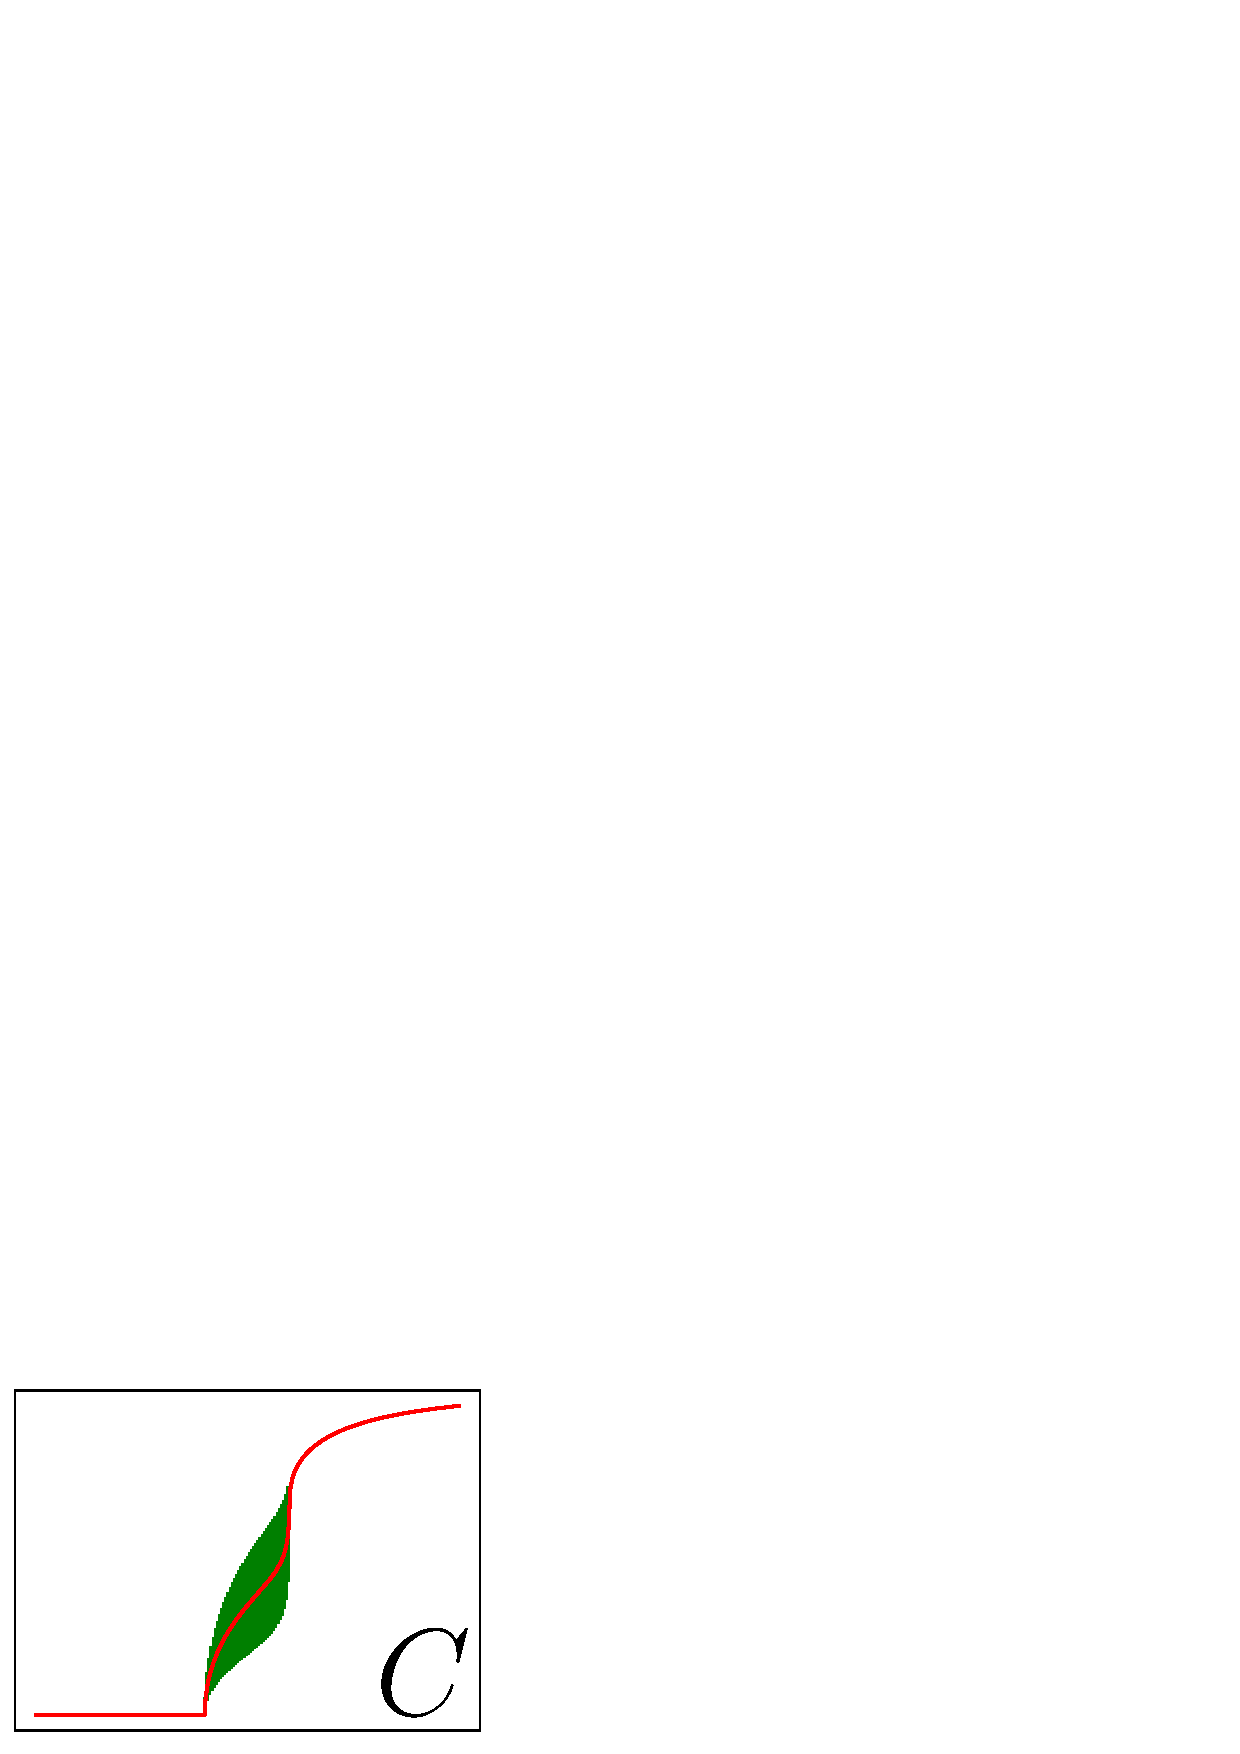
\includegraphics{C.pdf}}
%  \end{minipage}
%   &
%   \begin{minipage}{10mm}
%    \scalebox{0.2}{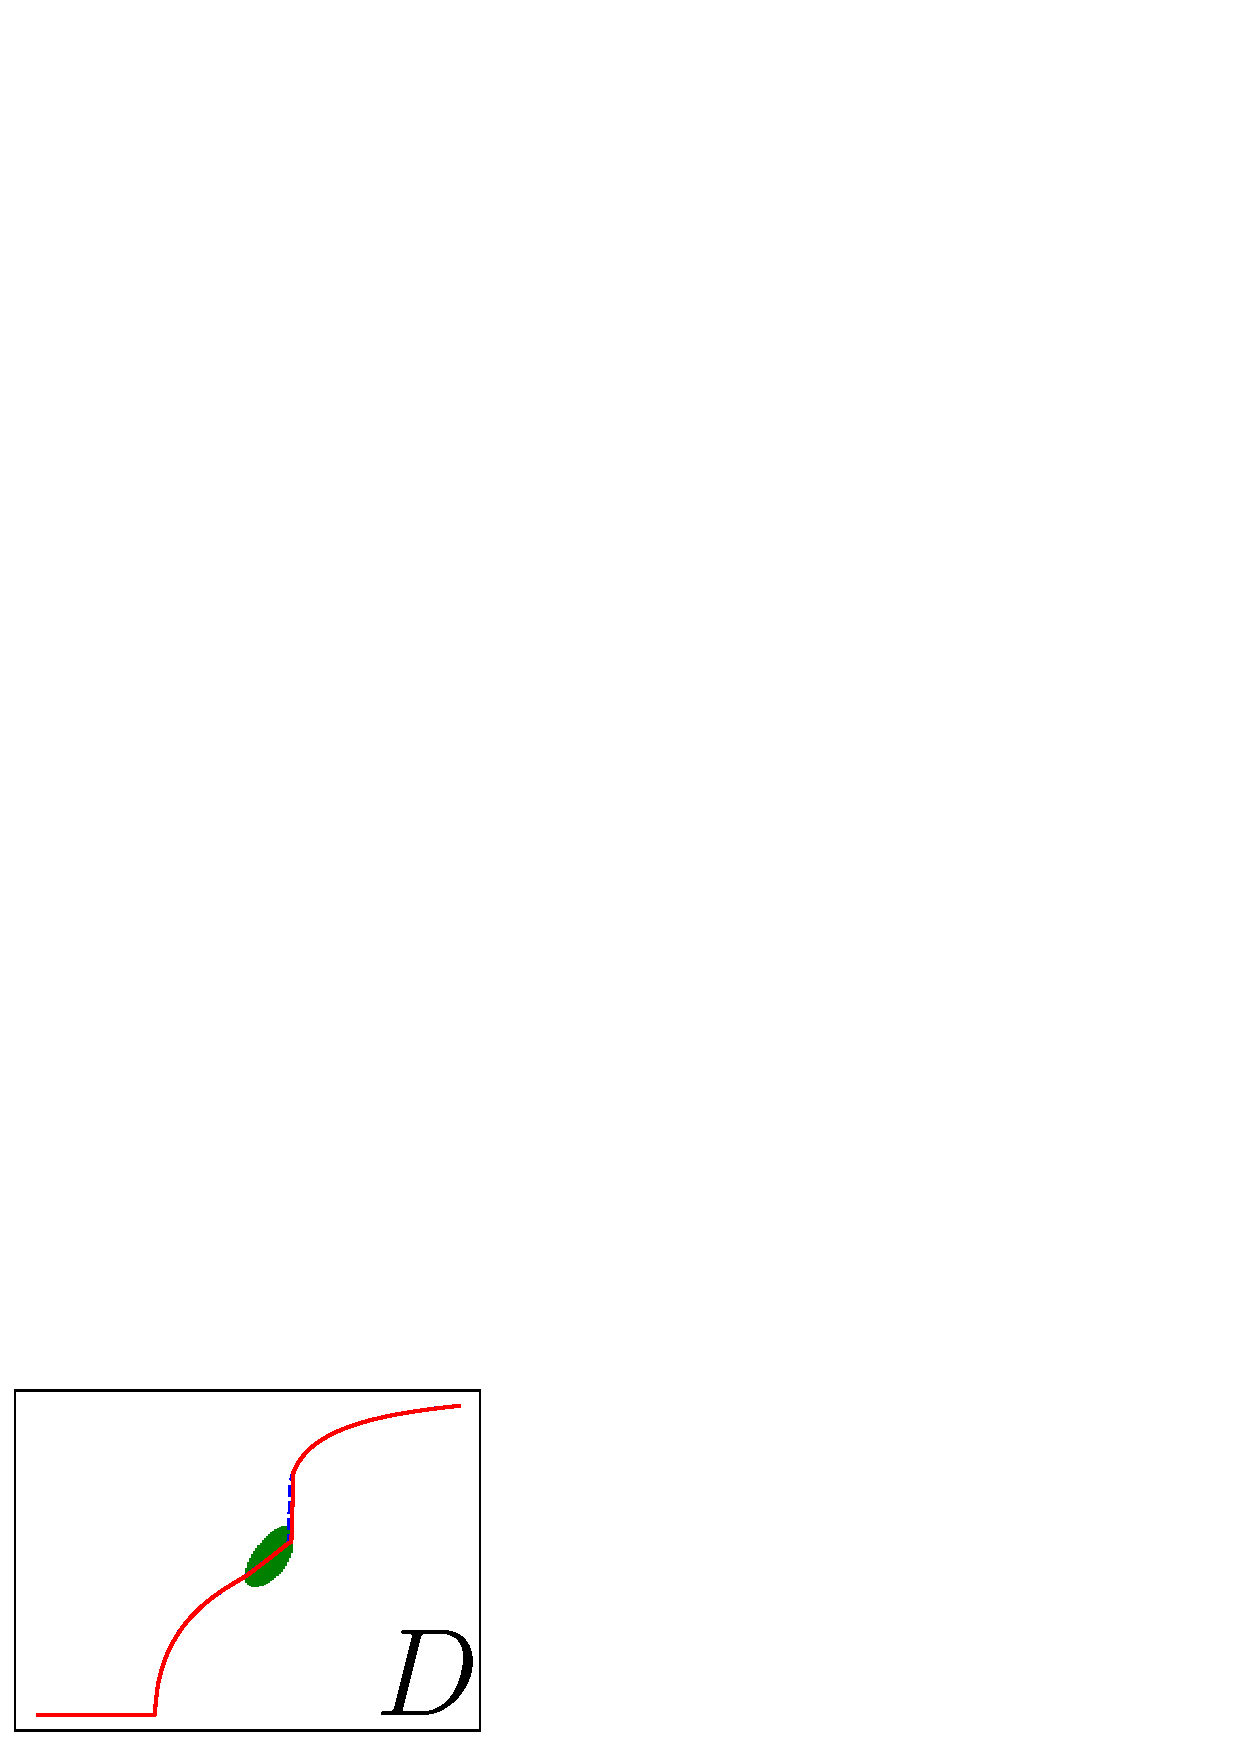
\includegraphics{D.pdf}}
%  \end{minipage}
%   &
%   \begin{minipage}{10mm}
%    \scalebox{0.2}{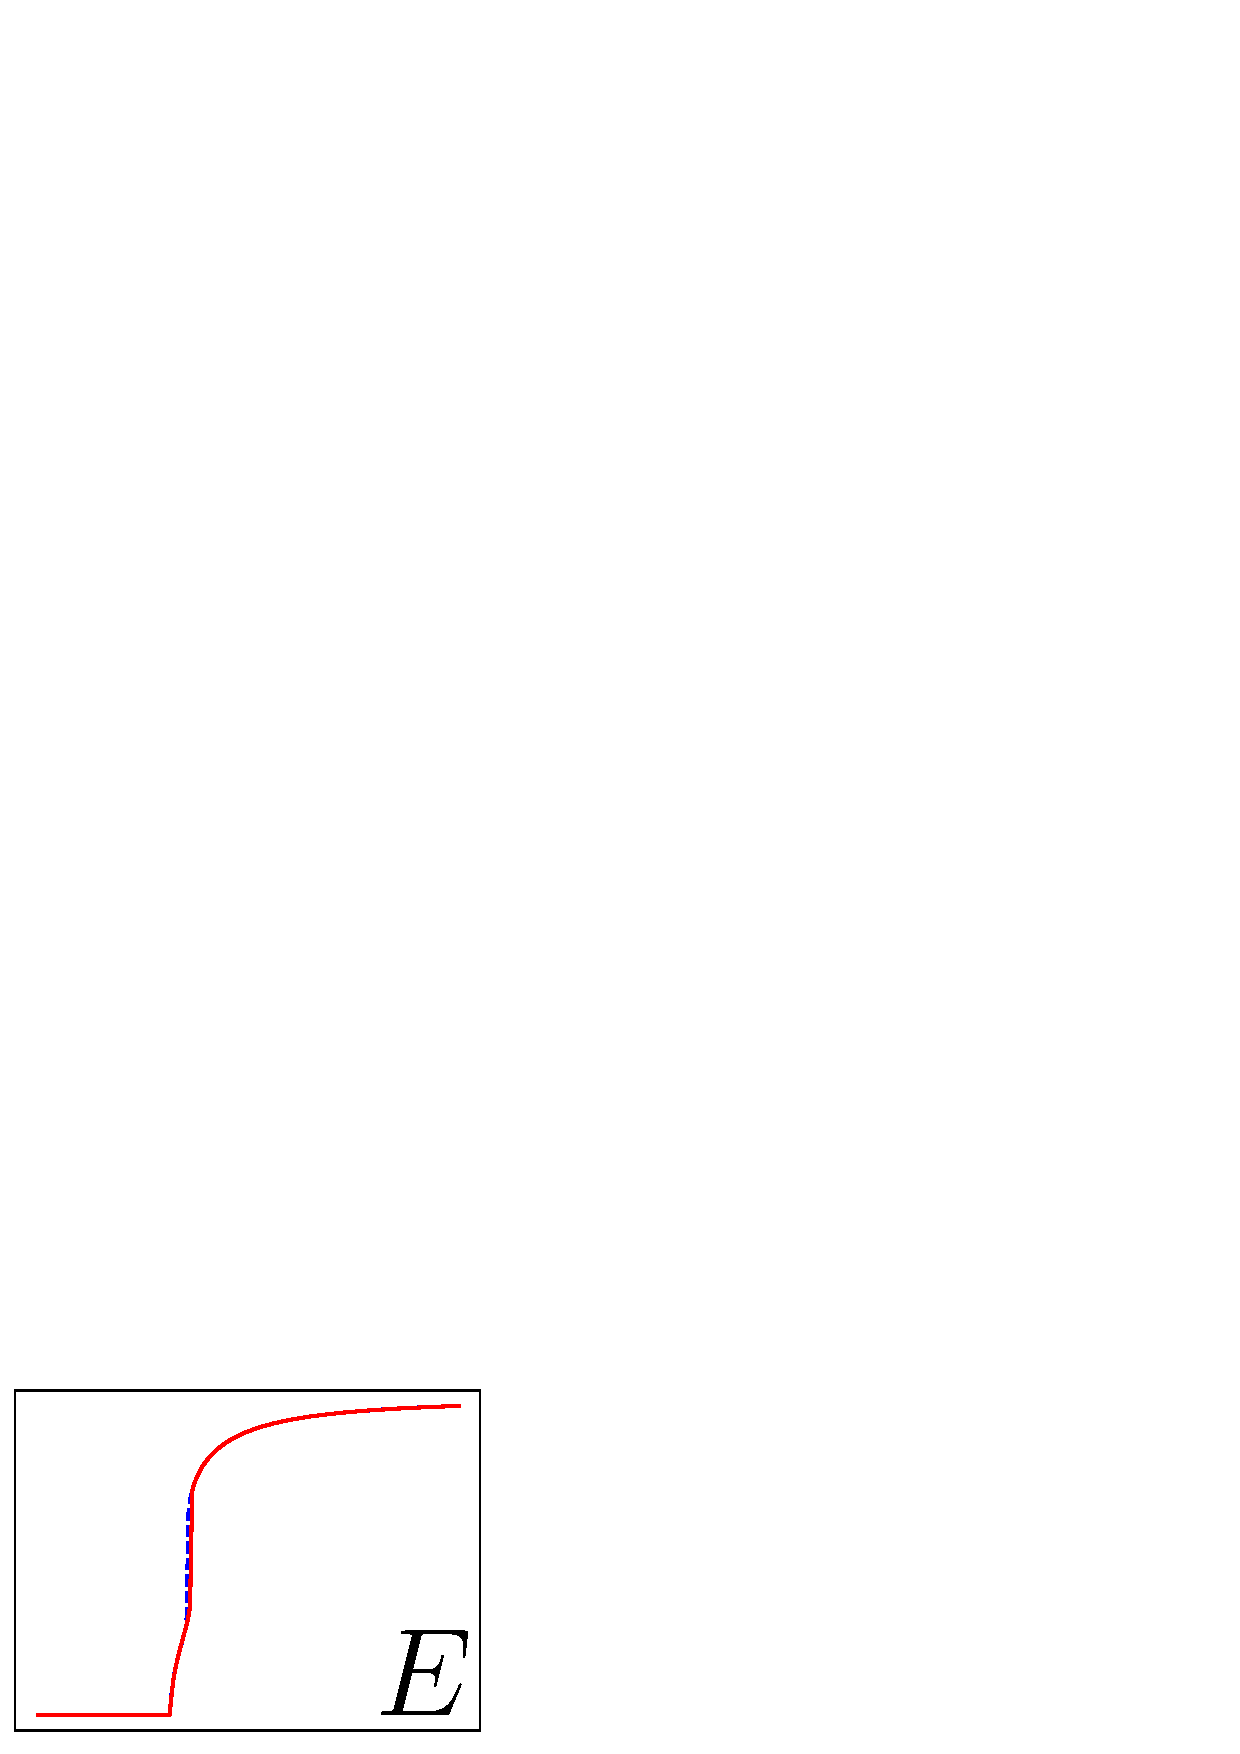
\includegraphics{E.pdf}}
%  \end{minipage}
%   \\\hline\hline
%  Linear~($\lambda_{1}$) & \checkmark & & \checkmark & \checkmark & \checkmark \\\hline
%  Nonlinear~($c_{3}$) & \checkmark & \checkmark & & \checkmark & \checkmark \\\hline
%  Nonlinear~($c_{5}$) & \checkmark & & & \checkmark & \checkmark \\\hline
%  Phenomenology & \checkmark & & \checkmark & \checkmark & \\\hline
%  \end{tabular}
%\end{table}

\begin{table}
  %\red{
  \caption{Techniques we use to determine the domains.
  $\lambda_{1}$ corresponds to the linear theory, and
  $c_{3}$ and $c_{5}$ correspond to the nonlinear theory.
  }
  \label{table:tech-domain}
  \begin{tabular}{c||c|c|c|c}
   & $\lambda_{1}$ & $c_{3}$ & $c_{5}$ & Phenomenology \\\hline\hline
   \begin{minipage}{20mm}
    \scalebox{0.2}{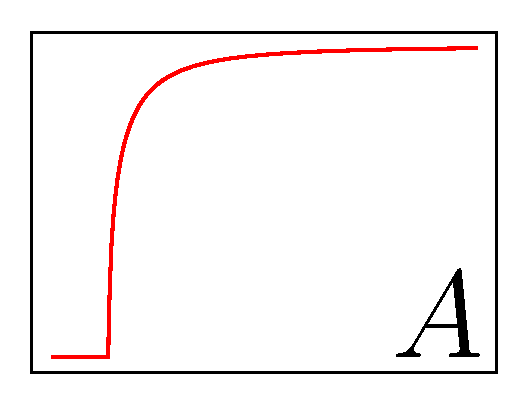
\includegraphics{figs/A.eps}}
  \end{minipage}
  & \checkmark & \checkmark & \checkmark & \checkmark \\\hline
  \begin{minipage}{20mm}
    \scalebox{0.2}{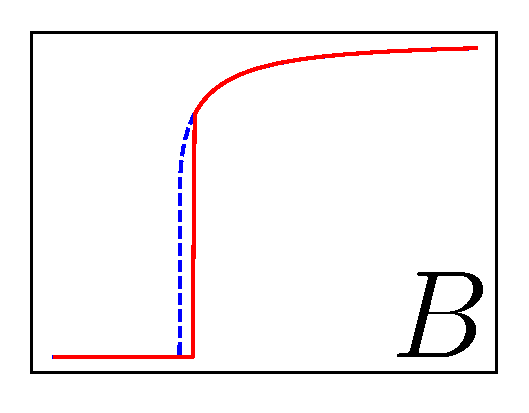
\includegraphics{figs/B.eps}}
  \end{minipage}
   & \checkmark & & & \\\hline
   \begin{minipage}{20mm}
    \scalebox{0.2}{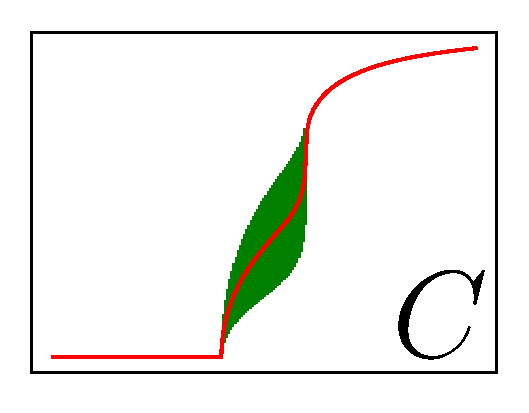
\includegraphics{figs/C.eps}}
  \end{minipage}
   & \checkmark & & & \checkmark \\\hline
   \begin{minipage}{20mm}
    \scalebox{0.2}{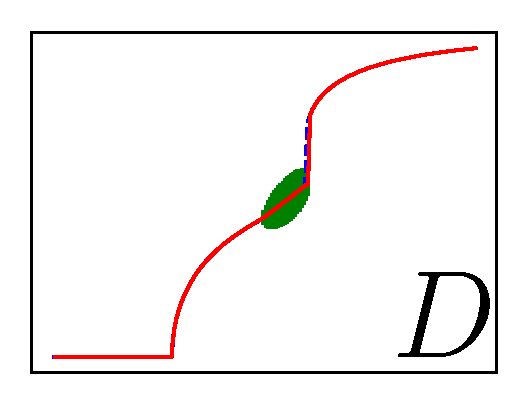
\includegraphics{figs/D.eps}}
  \end{minipage}
   & \checkmark & \checkmark & \checkmark & \checkmark \\\hline
   \begin{minipage}{20mm}
    \scalebox{0.2}{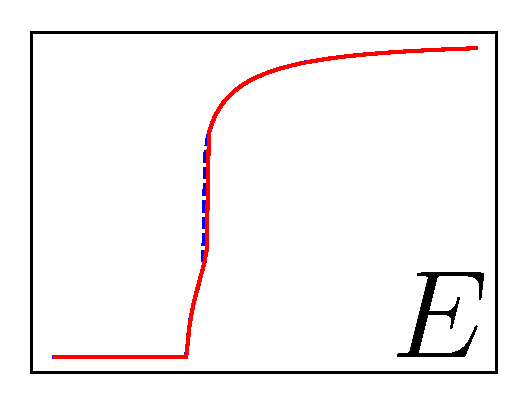
\includegraphics{figs/E.eps}}
  \end{minipage}
   & \checkmark & \checkmark & \checkmark & \\\hline
  \end{tabular}
  %}
\end{table}

The flow proposed above provides three theoretical lines,
I, II, and III
which divide the parameter plane $(\gamma_{1},\Omega)$ into the five domains,
as reported in Fig.~\ref{fig:pd-aa}.
%\red{In the region $\gamma_{1}<1$,
  the upper side of the line I is the theoretical domain D,
  the inside of the line II is the theoretical domain B,
  and the lines I, II, and III enclose the theoretical domain E.
%}
The theoretical lines reproduce qualitatively
the numerically obtained domains.

\begin{figure}[htbp]
\begin{center}
  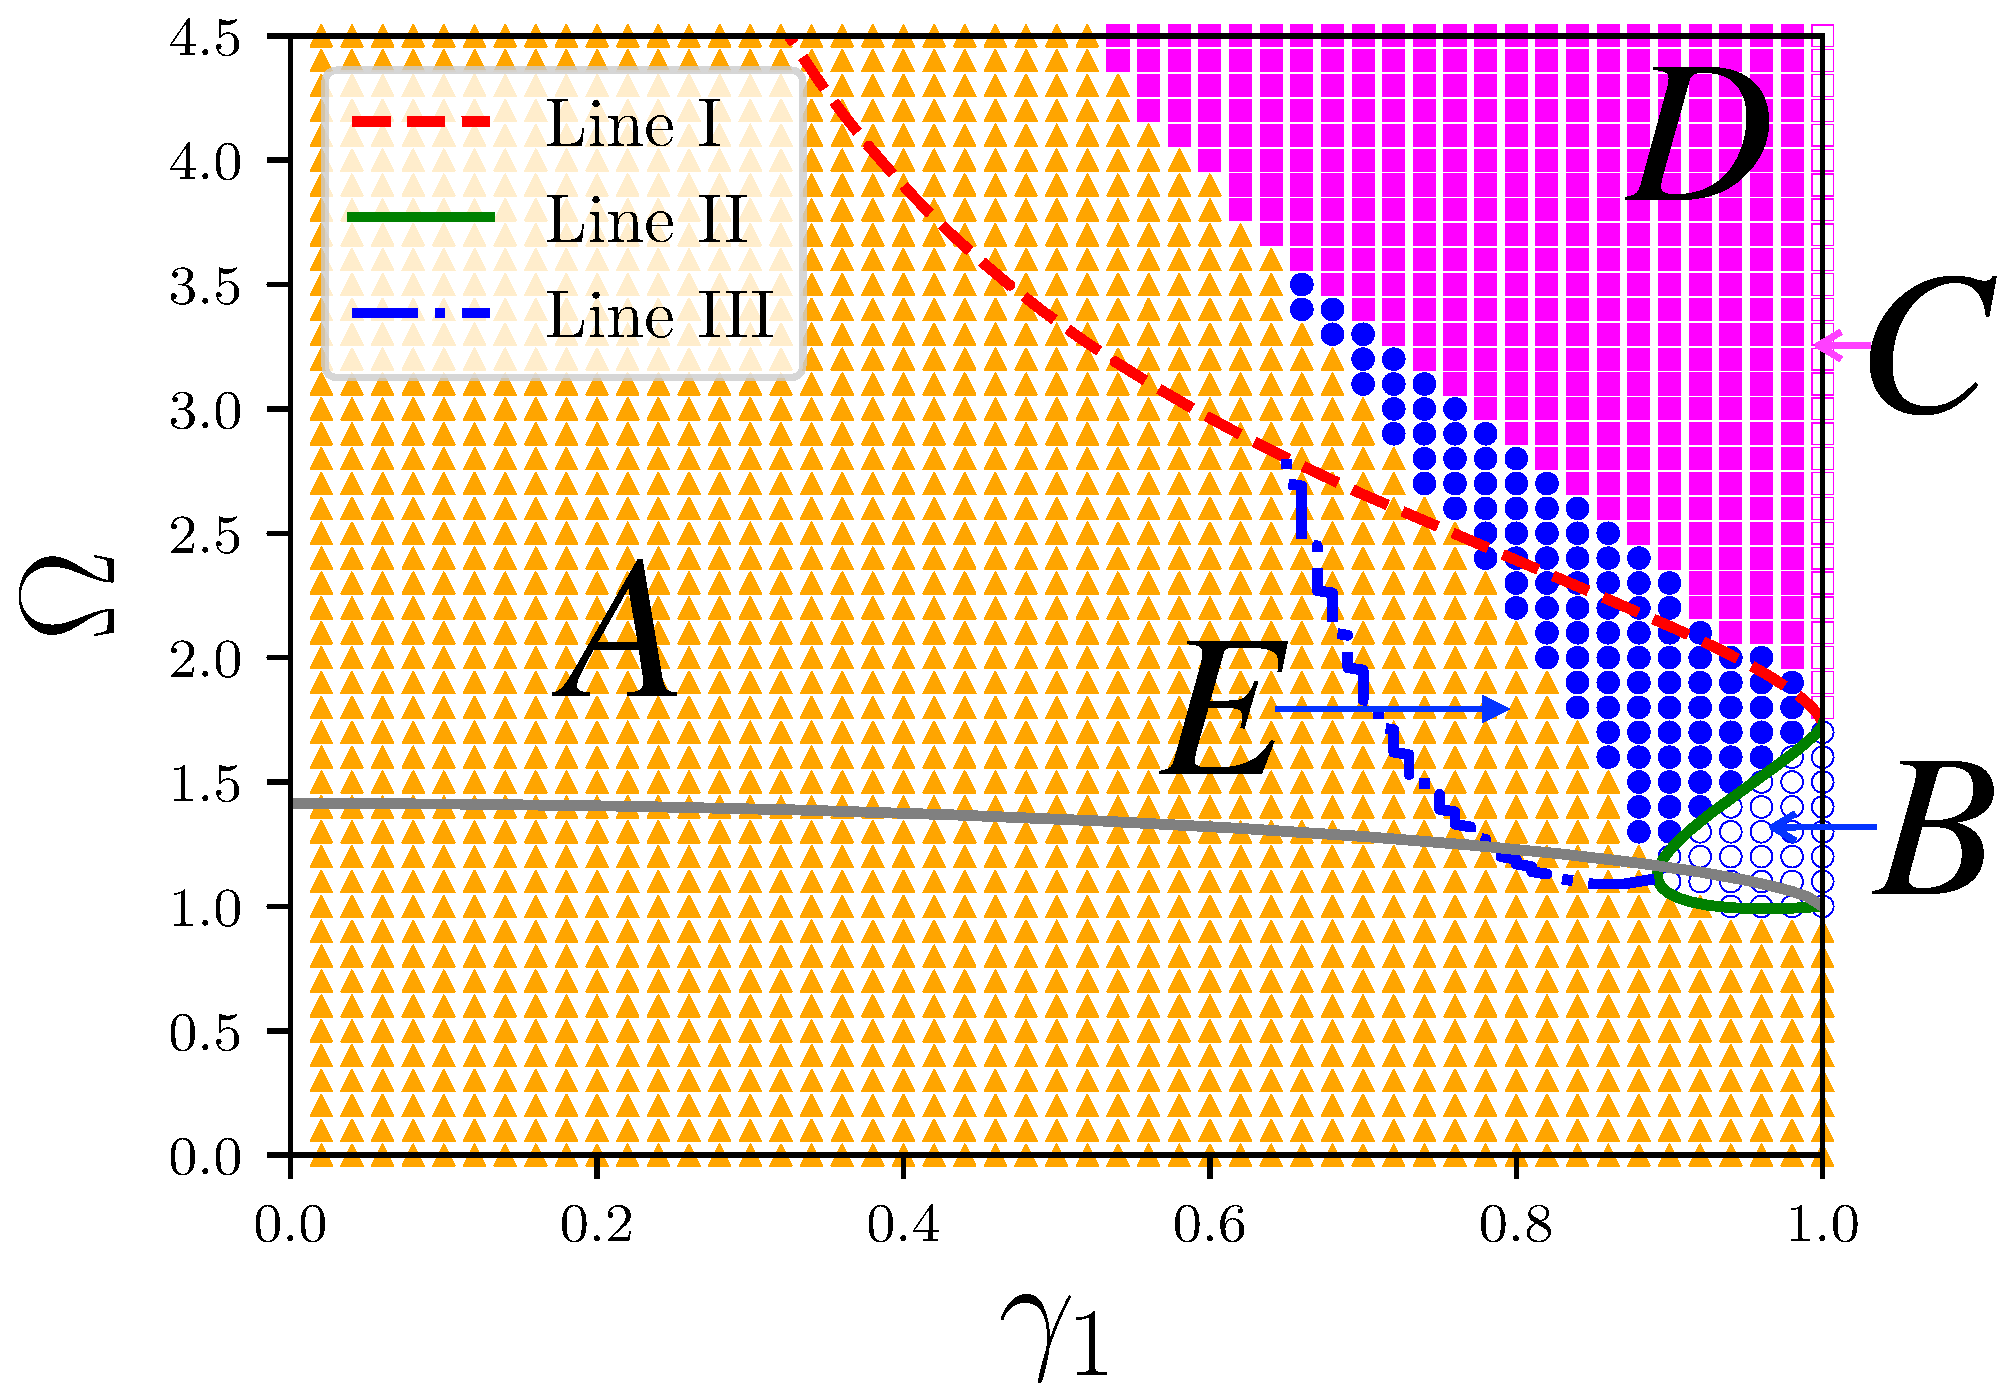
\includegraphics[width=8cm]{figs/pd-aa.eps}
\end{center}
\caption{
  %\red{Comparison between the theoretical and numerical classifications.
    The theoretical lines I(red broken line),
    II(green solid line), and III(blue dash-dotted line) are overlapped
    on Fig.~\ref{fig:phase-diagram}.
    % Theoretical classification of the parameter plane
    % overlapped on the Fig.~\ref{fig:phase-diagram}.
    %The domain B is perfectly enclosed by the line I.
    %The theoretical domain E is enclosed by  all the lines I, II, and III.
    Line I denotes the borderline between %the domain D and
    the domains D and ${\rm A}\cup{\rm B}\cup{\rm E}$.
    Line II denotes the borderline between %the domain B and domain A,C,E.
    the domains B and ${\rm A}\cup{\rm C}\cup{\rm E}$.
    Line III denotes the borderline between %the domain E and domain A.
    the domains E and A.
    The gray line represents the borderline between the unimodal and bimodal natural frequency distributions $g(\omega)$.
    %}
  %\blue{\it (I want the domain names in this figure.)}
  }
  \label{fig:pd-aa}
\end{figure}


% The line I is in good agreement with numerical results.
% This agreement is not supprising, because the asymmetry
% \red{separates the domain D from the domain C}
% and hence drawing the line I is not hard.
% {\it (Drop I?)}

For the line I, our result is fairly consistent with numerical ones,
but the domain D is overestimated.
Our method says that
the emergence of two clusters is associated with 
the emergence of two unstable eigenvalues.
% However, as we discussed previously,
% the second eigenvalue does not always
% give rise to the second cluster.
The second eigenvalue, however, does not always
  give rise to the second cluster as we discussed
  in Sec.~\ref{sec:oscillation}.
We have to reduce the domain D by introducing
an additional condition that
$|{\rm Im}(\lambda_{1}^{\ast})-{\rm Im}(\lambda_{2}^{\ast})|$
is sufficiently large.

The line II is perfect because the order parameter is small
around the critical point of the synchronization transition
and the perturbatively obtained amplitude equation is valid
for such a small amplitude.
This criterion had been used for symmetric $g(\omega)$,
but we have confirmed that it is also powerful for asymmetric ones.
The line II also reveals existence of discontinuous
synchronization transition for unimodal but asymmetric distributions.
The existence has been pointed out numerically in a previous study \cite{terada2018},
but our theoretical analysis ensures it.


% The line III is not perfect but captures the domain E qualitatively.
% As we expected, the theoretical prediction becomes precise around the domain B,
% and the performance is not ideal when not around the domain B.
% However this is not unexpected.
% In fact the absolute value of the order parameter 
% at $K_{\mathrm{Q}}$ gets bigger
% when the $\gamma_{1}$ gets smaller.
% Numerical simulations supports this in Fig.~\ref{fig:jump},
% for $\Omega=1.7$ and $\gamma_{1}\in[0.85,1.0]$.

The line III is not perfect.
We used a perturbative method to derive the amplitude equation
\eqref{eq:amplitude-equation-complex},
assuming that the order parameter is sufficiently small
at the jumping point $K_{\rm Q}$.
This assumption becomes worse as the point $(\gamma_{1},\Omega)$
approaches to the boundary of the domain E
where the width of the hysteresis vanishes
as reported in Fig.~\ref{fig:jump}.
It is thus expectable that the boundary of the domain E
is not perfectly described by the theoretical line III.
Nevertheless, the theoretical line III captures the domain E qualitatively
and is useful to have a strong candidate of the domain E.
% We remark that the theoretical prediction is easier
% than direct numerical detection
% because the latter requires to use a sufficiently small step of $K$
% to find the histerisis arond the boundary,
% while the small step is not necessary in the theory
% with the aid of the intermediate value theorem.

% \red{
% Nevertheless, the theoretical line III is useful to find the domain E
% because it captures the domain E qualitatively
% and gives a strong candidate of the domain E easily.
% We underline that numerical finding of the domain E
% gets harder as $\gamma_{1}$ decreases
% because the width of the histerisis shrinks as shown in Fig.~\ref{fig:jump}.
% We thus have to use a sufficiently small step of $K$
% to detect the histerisis from the forward and backward processes.
% The theoretical criterion is, on the contrary,
% existence of a zero point of the discriminant $\Delta(K)$,
% and the existence can be easily guaranteed 
% by the intermediate value theorem.
% }




\begin{figure}
\begin{center}
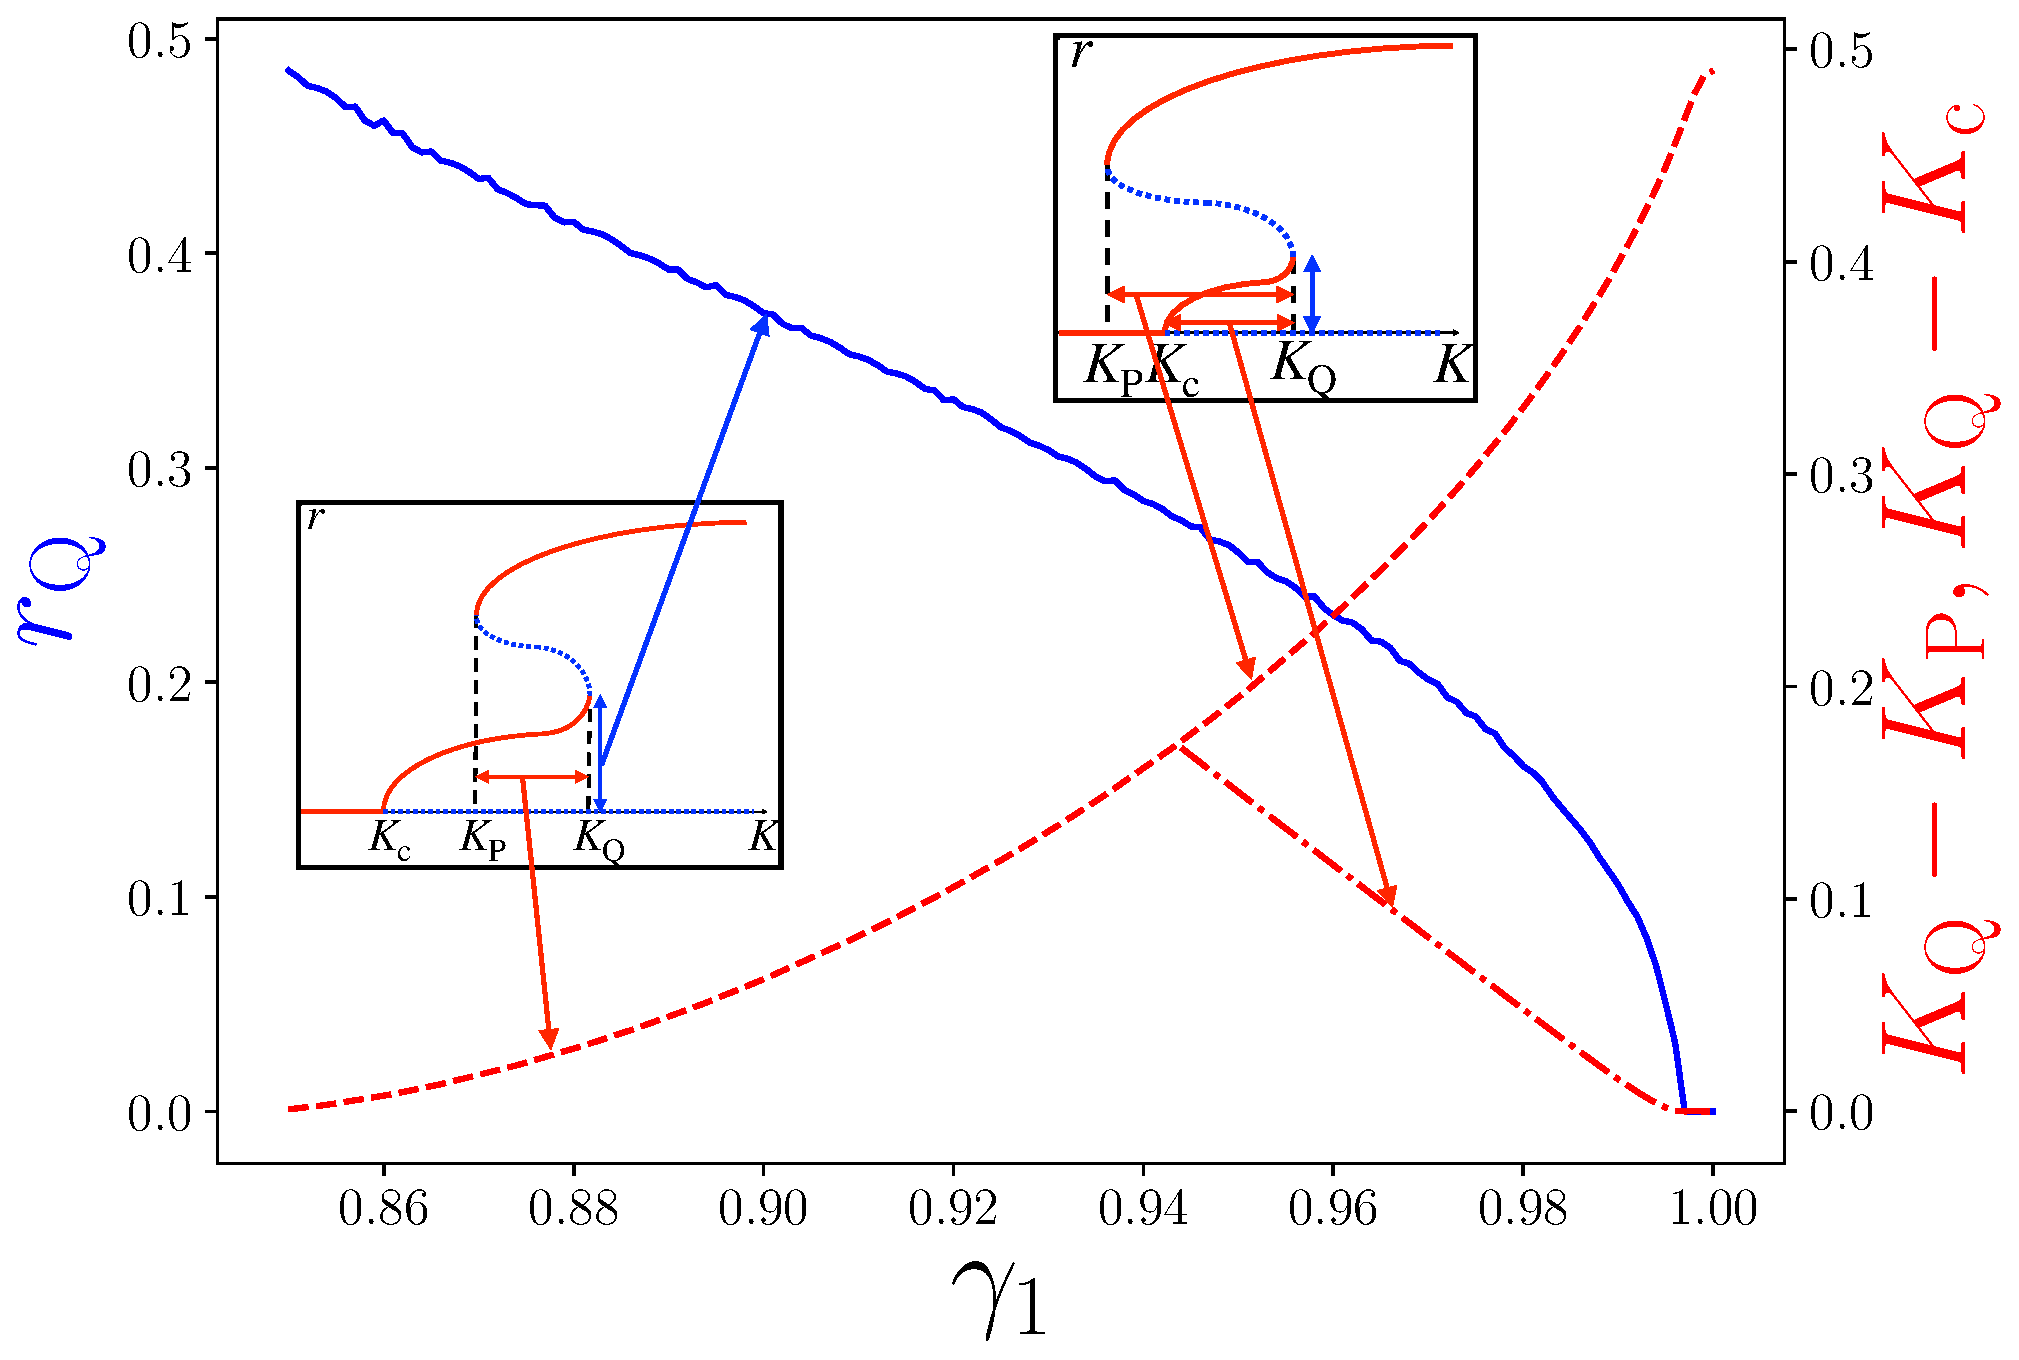
\includegraphics[width=8cm]{figs/jump.eps}
\end{center}
\caption{The absolute value $r$ of the order parameter
  at $K_{\mathrm{Q}}$(blue solid line)
  and the value $K_{\mathrm{Q}}-K_{\mathrm{P}}$(red dashed line)
  for $\Omega=1.7$.
  As $\gamma_{1}$ decreases,
  $r_{\mathrm{Q}}$, the smaller value of $r$ at $K=K_{\mathrm{Q}}$,
  increases monotonically,
  and the value $K_{\mathrm{Q}}-K_{\mathrm{P}}$
  decreases monotonically.
  The red dash-dotted line represents the value
  $K_{\mathrm{Q}}-K_{\mathrm{c}}$,
  which is drawn only for $\gamma_{1}$ giving $K_{\mathrm{P}}<K_{\mathrm{c}}$;
  The upper stable branch emerges
  before the lower unstable branch emerges.
  }
  \label{fig:jump}
\end{figure}

% We, therefore, conclude that the higher order analysis
% of the amplitude equation is useful to predict
% the discontinuous bifurcation emerging from a partially synchronized state.



\section{Conclusion and Discussions}
\label{sec:conclusion}

We have proposed a theoretical method to classify bifurcation diagrams
in the Kuramoto model
by using the amplitude equation with the aid of the linear analysis
around the nonsynchronized reference state.
The amplitude equation, obtained perturbatively,
is usually stopped up to the second leading term
because it is sufficient to judge the continuity
of the synchronization transition, bifurcation from the nonsynchronized state.
The premise, however, is broken by introducing asymmetry
  in the natural frequency distribution
  because the asymmetry induces bifurcations from partially synchronized states.
% Asymmetry in the natural frequency distribution introduces
% bifurcations from partially synchronized states
%and the second leading term is not sufficient to characterize them.
We have extended the amplitude equation up to the third leading term
and successfully captured a discontinuous bifurcation after a continuous one.

For bifurcation diagrams having oscillating states,
we have focused on unstable eigenvalues of the nonsynchronized state.
Roughly speaking, one unstable eigenvalue corresponds to one cluster formation,
and hence existence of two unstable eigenvalues suggest
appearance of two clusters rotating with different speeds.
This idea is qualitatively in good agreement with numerical results,
but overestimates the domain having the oscillation.
We have to reduce the domain by adding one more condition
which requires a large discrepancy of rotating speeds of the two clusters
in order to avoid the absorption of the second virtual cluster
by the first grown cluster.
The additional condition has to be investigated.
We remark that a similar condition was discussed in a Hamiltonian system
\cite{barre-yamaguchi-09}.

%\red{
%  In this paper,
  We mainly used the amplitude equation to predict the bifurcation diagram.
%  We have to note that
  This method is a perturbation technique
  and is not powerful if the considering point is far from the critical point.
  This restriction prevents us from getting precise theoretical lines
  for $\Omega$ sufficiently large, for instance, because the oscillation/jump
  emerging from a partially synchronized state are not close to the critical point.
  On the contrary, for symmetric and bimodal natural frequency distributions,
  our method successfully identified the oscillating states,
  the domain C, solely by a linear analysis with phenomenology,
  while they have been previously analyzed by a nonlinear analysis,
  the amplitude equation \cite{crawford1994}.
  Our analysis hence captures an essence of the oscillating states.
%}

It is worth noting that a cluster is created by
the resonance between natural frequencies an unstable eigenvalue,
but the number of clusters, $n_{c}$,
is not necessarily the same with the number of unstable eigenvalues, $n_{u}$.
In our computations, $n_{c}=1$ when $n_{u}=1$
but $n_{c}\geq 2$ when $n_{u}=2$.
Such a multi-cluster state with $n_{c}>2$, called the Bellerophon state, 
was reported previously \cite{bi2016,li2019}
but the mechanism is an open question.
Noting that two or more clusters induce oscillation of the order parameter
and following the scenario that a resonance makes a cluster,
we expect that the multi-cluster state with $n_{c}>2$
is realized hierarchically by resonances between natural frequencies
and the frequencies of the order parameter oscillation.
This scenario has to be investigated.


Finally, we discuss applications of our theory
to general coupled oscillator models.
Introducing the phase-lag parameter in the coupling function
\cite{sakaguchi-kuramoto-86},
we have a phase diagram having a continuous synchronization transition
followed by a discontinuous jump as the type E
\cite{omelchenko-wolfrum-12}.
Analyzing this system is a straightforward application of our theory.
Studying time delay \cite{yeung-strogatz-99,montbrio-pazo-schmidt-06}
is also an interesting application.
If the coupling function becomes general,
the coefficients of the amplitude equation may have
divergences as the coupling constant goes to the critical value
%\red{
  as shown in a collisionless plasma \cite{crawford1995b}.
%}
%\cite{crawford1995}.
For instance, the coefficient ${\rm Re}(c_{3})$ may be proportional to
a power of $1/{\rm Re}(\lambda_{1})$.
%\red{
  Nevertheless, the amplitude equation captures the asymptotic
  scaling of the order parameter against the strength of instability
  in plasmas, and we may expect that the amplitude equation still has power
  to predict the bifurcation diagram.
%}
It is another future problem to check
%whether the proposed criterion is persistent under such divergences of coefficients.
the precision of the proposed criterion under such divergent coefficients.


% \appendix


\begin{thebibliography}{99}
%\bibitem{bennett2002}
%  M. Bennett, M. F. Scatz, H. Rockwood, and K. Wiesenfeld, Huygen's clocks, \textit{Proc. R. Soc. London A} \textbf{458}, 563 (2002).
\bibitem{pantaleone2002}
  J. Pantaleone, Synchronization of metronomes, \textit{Am. J. Phys.} \textbf{70}, 992 (2002).
\bibitem{smith1935}
  H. M. Smith, Synchronous flashing of fireflies, \textit{Science} \textbf{82}, 151 (1935).
\bibitem{buck1968}
  J. Buck and E. Buck, Mechanism of rhythmic synchronous flashing of fireflies, \textit{Science} \textbf{159}, 1319 (1968).
\bibitem{aihara2014}
  I. Aihara, T. Mizumoto, T. Otsuka, H. Awano, K. Nagira, H. G. Okuno and K. Aihara,
  Spatio-Temporal Dynamics in Collective Frog Choruses Examined by Mathematical Modeling and Field Observations,
  \textit{Sci. Rep.} {\bf 4}, 3891 (2014).
\bibitem{wiesenfeld1996}
  K. Wiesenfeld, P. Colet and S. H. Strogatz,
  Synchronization Transitions in a Disordered Josephson Series Array,
  \textit{Phys. Rev. Lett.} {\bf 76}, 404 (1996).
\bibitem{wiesenfeld1998}
  K. Wiesenfeld, P. Colet and S. H. Strogatz,
  Frequency locking in Josephson arrays: Connection with the Kuramoto model,
  \textit{Phys. Rev. E} {\bf 57}, 1563 (1998).
\bibitem{winfree1967}
  A. T. Winfree,
  Biological Rhythms and the Behavior of Populations of Coupled Oscillators,
  \textit{J. Theoret. Biol.} {\bf 16}, 15 (1967).
\bibitem{kuramoto1975}
  Y. Kuramoto, Self-entertainment of a population of coupled non-linear oscillators, \textit{International Symposium on Mathematical Problems in Theoretical Physics, Lecture Notes in Physics} \textbf{39}, 420 (1975).
\bibitem{strogatz2000}
  S. H. Strogatz, From Kuramoto to Crawford: exploring the onset of synchronization in populations of coupled oscillators, \textit{Physica} \textbf{143D}, 1 (2000).
\bibitem{chiba2015}
  H. Chiba, A proof of the Kuramoto conjecture for a bifurcation structure of the infinite-dimensional Kuramoto model, \textit{Ergod. Theo. Dyn. Syst.} \textbf{35}, 762 (2015).

\bibitem{basnarkov-urumov-07}
  L. Basnarkov and V. Urumov,
  Phase transitions in the Kuramoto model,
  \textit{Phys. Rev. E} \textbf{76}, 057201 (2007).
  
\bibitem{bastian-18}
  B. Pietras, N. Deschle, and A. Daffertshofer,
  First-order phase transitions in the Kuramoto model with compact bimodal frequency distributions,
  \textit{Phys. Rev. E} \textbf{98}, 062219 (2018).
  
% \bibitem{bonilla-neu-spigler-92}
%   \red{
%     L. L. Bonilla, J. C. Neu, and R. Spigler,
%   Nonlinear Stability of Incoherence and Collective Synchronization in a Population of Coupled Oscillators,
%   J. Stat. Phys. {\bf 67}, 313 (1992).
%   }


\bibitem{martens2009}
  E. A. Martens, E. Barreto, S. H. Strogatz, E. Ott, P. So, and T. M. Antonsen, Exact results for the Kuramoto model with a bimodal frequency distribution, \textit{Phys. Rev. E} \textbf{79}, 026204 (2009).

\bibitem{terada2017}
  Y. Terada, K. Ito, T. Aoyagi, and Y. Y. Yamaguchi, Nonstandard transition in the Kuramoto model: a role of asymmetry in natural frequency distributions, \textit{J. Stat. Mech.} (2017) 0134403.

\bibitem{pazo-05}
  D. Paz\'{o},
  Thermodynamic limit of the first-order phase transition in the Kuramoto model,
  \textit{Phys. Rev. E} {\bf 72}, 046211 (2005).

\bibitem{park-kahng-19}
  J. Park and B. Kahng,
  Synchronization transitions through metastable state on structured networks,
  arXiv:1901.02123.

\bibitem{komarov-pikovsky-13}
  M. Komarov and A. Pikovsky,
  Multiplicity of Singular Synchronous States in the Kuramoto Model of Coupled Oscillators,
  \textit{Phys. Rev. Lett.} {\bf 111}, 204101 (2013).

\bibitem{komarov-pikovsky-14}
  M. Komarov and A. Pikovsky,
  The Kuramoto model of coupled oscillators with a bi-harmonic coupling function,
  \textit{Physica D} {\bf 289}, 18 (2014).

\bibitem{oa2008}
  E. Ott and T. M. Antonsen, Low dimensional behavior of large systems of globally coupled oscillators, \textit{Chaos} \textbf{18}, 037113 (2008).

\bibitem{oa2009}
  E. Ott and T. M. Antonsen,
  Long time evolution of phase oscillator systems,
  \textit{Chaos} {\bf 19}, 023117 (2009).

\bibitem{lu-etal-16}
  % Zhixin Lu, Kevin Klein-Carde\~{n}a, Steven Lee, Thomas M. Antonsen, Michelle Girvan, and Edward Ott,
  Z. Lu, K. Klein-Carde\~{n}a, S. Lee, T. M. Antonsen, M. Girvan, and E. Ott,
  Resynchronization of circadian oscillators and the east-west asymmetry of jet-lag,
  \textit{Chaos} \textbf{26}, 094811 (2016).
  
\bibitem{akao-19}
  % Akihiko Akao, Sho Shirasaka, Yasuhiko Jimbo, Bard Ermentrout and Kiyoshi Kotani,
  A. Akao, S. Shirasaka, Y. Jimbo, B. Ermentrout, and K. Kotani,
  Theta-gamma cross-frequency coupling enables covariance between distant brain regions,
  arXiv:1903.12155.

\bibitem{crawford1994}
  J. D. Crawford, Amplitude Expansions for Instabilities in Populations of Globally-Coupled Oscillators, 
  %\textit{J. \red{Stat.} Phys.} 
  \textit{J. Stat. Phys.} 
  \textbf{74}, 1047 (1994). 

\bibitem{crawford1995}
  J. D. Crawford,
  Scaling and Singularities in the Entrainment of Globally Coupled Oscillators,
  {\it Phys. Rev. Lett.} {\bf 74}, 4341 (1995).

\bibitem{metivier-19}
  D. M\'{e}tivier and S. Gupta,
  Bifurcations in the Time-Delayed Kuramoto Model of Coupled Oscillators: Exact Results,
  \textit{J. Stat. Phys.}, (2019).
  
  
\bibitem{barre2016}
  J. Barr\'{e} and D. M\'{e}tivier, Bifurcations and Singularities for Coupled Oscillators with Inertia and Frustration, \textit{Phys. Rev. Lett.} \textbf{117}, 214102 (2016).

\bibitem{crawford1994b}
  J. D. Crawford,
  Universal Trapping Scaling on the Unstable Manifold for a Collisionless Electrostatic Mode,
  {\it Phys. Rev. Lett.} {\bf 73}, 656 (1994).

\bibitem{crawford1995b}
  J. D. Crawford,
  Amplitude equations for electrostatic waves: Universal singular behavior in the limit of weak instability,
  {\it Phys. Plasmas} {\bf 2}, 97 (1995).

\bibitem{barre-metivier-yamaguchi-16}
  J. Barr{\'e}, D. M{\'e}tivier, and Y. Y. Yamaguchi,
  Trapping scaling for bifurcations in the Vlasov systems,
  \textit{Phys. Rev. E} {\bf 93}, 042207 (2016).


\bibitem{hansel-mato-meunier-93}
  D. Hansel, G. Mato and C. Meunier,
  Phase Dynamics for Weakly Coupled Hodgkin-Huxley Neurons,
  \textit{Europhys. Lett.} {\bf 23}, 367 (1993).

\bibitem{kiss-zhai-hudson-05}
  I. Z. Kiss, Y. Zhai and J. L. Hudson,
  Predicting Mutual Entrainment of Oscillators with Experiment-Based Phase Models,
  \textit{Phys. Rev. Lett.} {\bf 94}, 248301 (2005).

\bibitem{kiss-zhai-hudson-06}
  I. Z. Kiss, Y. Zhai and J. L. Hudson,
  Characteristics of Cluster Formation in a Population of Globally Coupled Electrochemical Oscillators: An Experiment-Based Phase Model Approach,
  \textit{Prog. Theor. Phys. Suppl.} {\bf 161}, 99 (2006).



\bibitem{terada2018}
  Y. Terada, K. Ito, R. Yoneda, T. Aoyagi and Y. Y. Yamaguchi,
  A role of asymmetry in linear response of globally coupled oscillator systems,
  arXiv:1802.08383.

\bibitem{lancellotti2004}
  C. Lancellotti, On the Vlasov Limit for Systems of Nonlinearly Coupled Oscillators without Noise, \textit{Transp. Theory Stat.} \textbf{34}, 523 (2004).


\bibitem{morita-kaneko-06}
  H. Morita and K. Kaneko,
  Collective Oscillation in a Hamiltonian System,
  \textit{Phys. Rev. Lett.} \textbf{96}, 050602 (2006).
  

  
  
%\bibitem{goldobin-etal-11}
%\red{
%  E. Goldobin, D. Koelle, R. Kleiner and R. G. Mints,
%  Josephson Junction with a Magnetic-Field Tunable Ground State,
%  Phys. Rev. Lett. {\bf 107}, 227001 (2011).
%}%

%\bibitem{goldobin-etal-13}
%\red{
%  E. Goldobin, R. Kleiner, D. Koelle and R. G. Mints,
%  Phase Retrapping in a Pointlike $\varphi$ Josephson Junction: The Butterfly Effect,
%  Phys. Rev. Lett. {\bf 111}, 057004 (2013).
%}%

%\bibitem{czolczynski-13}
%\red{
%  K. Czolczynski, P. Perlikovski, A. Stefanski and T. Kapitaniak,
%  Synchronization of the self-excited pendula suspended on the vertically displacing beam,
%  Commun. Nonlinear Sci. Numer. Simul. {\bf 18}, 386 (2013).
%}

%\bibitem{li-etal-14}
%\red{
%  K. Li, S. Ma, H. Li and J. Yang,
%  Transition to synchronization in a kuramoto model with the first- and second-order interaction terms,
%  Phys. Rev E {\bf 89}, 032917 (2014).
%}


  
\bibitem{barre-yamaguchi-09}
  J. Barr{\'e} and Y. Y. Yamaguchi,
  Small traveling clusters in attractive and repulsive Hamiltonian mean-field models,
  \textit{Phys. Rev. E} {\bf 79}, 036208 (2009).

\bibitem{bi2016}
H. Bi, X. Hu, S. Boccaletti, X. Wang,
Y. Zou, Z. Liu, and S. Guan,
Coexistence of Quantized, Time Dependent, Clusters in Globally Coupled Oscillators,
\textit{Phys. Rev. Lett.} \textbf{117}, 204101 (2016).

\bibitem{li2019}
X. Li, T. Qiu, S. Boccaletti,
I. Sendi-Nadal, Z. Liu and S. Guan,
Synchronization clusters emerge as the result of a global coupling among classical phase oscillators,
\textit{New J. Phys.} \textbf{21}, 053002 (2019).

\bibitem{sakaguchi-kuramoto-86}
  H. Sakaguchi and Y. Kuramoto,
  A Soluble Active Rotator Model Showing Phase Transitions via Mutual Entrainment,
  \textit{Prog. Theor. Phys.} {\bf 76}, 576 (1986).

\bibitem{omelchenko-wolfrum-12}
  O. E. Omel'chenko and M. Wlfrum,
  Nonuniversal Transitions to Synchrony in the Sakaguchi-Kuramoto Model,
  \textit{Phys. Rev. Lett.} {\bf 109}, 164101 (2012).

\bibitem{yeung-strogatz-99}
  M. K. S. Yeung and S. H. Strogatz,
  Time Delay in the Kuramoto Model of Coupled Oscillators,
  \textit{Phys. Rev. Lett.} {\bf 82}, 648 (1999).

\bibitem{montbrio-pazo-schmidt-06}
  E. Montbri{\'o}, D. Paz{\'o} and J. Schmidt,
  Time delay in the Kuramoto model with bimodal frequency distribution,
  \textit{Phys. Rev. E} {\bf 74}, 056201 (2006).

\bibitem{strogatz1992}
  S. H. Strogatz, R. E. Mirollo and P. C. Matthews,
  Coupled Nonlinear Oscillators below the Synchronization Threshold: Relaxation be Generalized Landau Damping,
  \textit{Phys. Rev. Lett.} {\bf 68}, 2730 (1992).

\bibitem{ogawa2013}
  S. Ogawa,
  Spectral and formal stability criteria of spatially inhomogeneous stationary solutions to the Vlasov equation for the Hamiltonian mean-field model,
  \textit{Phys. Rev. E} {\bf 87}, 062107 (2013). 



\begin{comment}
\bibitem{mirollo1990}
  R. E. Mirollo and S. H. Strogatz, Amplitude Death in an Array of Limit-Cycle Oscillations, \textit{J. Statist. Phys.} \textbf{60}, 245 (1990).
\bibitem{strogatz1990}
  S. H. Strogatz and R. E. Mirollo, Stability of Incoherence in a Population of Coupled Oscillators, \textit{J. Statist. Phys.} \textbf{63}, 613 (1991).
\bibitem{sakaguchi1988}
  H. Sakaguchi, Cooperative phenomena in coupled oscillator systems under external fields, \textit{Prog. Theor. Phys.} \textbf{79}, 39 (1988).
\bibitem{komarov2013}
  M. Komarov and A. Pikovsky, Multiplicity of Singular Synchronous States in the Kuramoto Model of Coupled Oscillators, \textit{Phys. Rev. Lett.} \textbf{111}, 204101 (2013).
\end{comment}

\end{thebibliography}